%========================================================================
% Modelo para elaboracao de textos academicos: TCC, dissertacoes e teses
% Elaborado pelo GISIS - Grupo de Imageamento Sismico e Inversao Sismica.
%========================================================================
\chapter{Metodologia}
\label{ch:metodologia}

Todas as informações dos experimentos realizados para verificar a precisão e a performance dos métodos de resolução da equação eikonal estão descritas neste capítulo. Começando pela comparação de precisão e performance utilizando modelos de propriedades simples e complexos, para averiguar a precisão em um modelo homogêneo, em um modelo de duas camadas e em um modelo complexo amplamente utilizado em análises sísmicas. Finalizando o capítulo, as estratégias da inversão tomográfica são discutidas, elucidando a construção do modelo inicial e de referência, a geometria de aquisição e a confecção do dado observado.

\section{Experimentos comparativos de modelagem}

Os resultados de performance são gerados no mesmo computador tendo um processador Intel i7-12700 com 20 núcleos e uma placa gráfica NVIDIA GeForce RTX 3060 com 12 GB de armazenamento. O sistema operacional Windows 11 é utilizado com a virtualização da distribuição linux Ubuntu via WSL.  

\subsection{Aplicação em modelo homogêneo}

Um modelo homogêneo foi aplicado com velocidade constante de 2000 m/s. O modelo tem 200 $\times$ 200 $\times$ 200 metros, com parâmetro de discretização de 1 m, totalizando 201 amostras em cada direção $x$, $y$ e $z$. A posição da fonte se encontra no centro do modelo. O tempo analítico é calculado a partir da distância da fonte a cada ponto da malha dividido pela velocidade do modelo. O erro é computado a partir da diferença entre o tempo numérico e o tempo analítico. As formulações de \citeonline{podvin1991finite}, \citeonline{jeong2008fast} e \citeonline{noble2014accurate} são analisadas. Como caso adicional, o operador mais preciso desenvolvido no trabalho de \citeonline{cai2023improved} é testado, pois o código foi fornecido pelo autor exatamente com um teste analítico nesse formado em questão. Como resultado, somente a média e o máximo erro são mostrados como no experimento de \citeonline{cai2023improved}. 

\subsection{Aplicação em modelo de refração}

Como parte de um experimento apresentado ao Simpósio Brasileiro de Geofísica \cite{alves2022refraction}, uma comparação numérica entre os métodos estudados será abordada, agora demonstrando a precisão no cálculo de ondas refratadas e o comportamento utilizando o princípio da reciprocidade. O exemplo esquemático aloca uma fonte na superfície do centro do modelo de velocidade e um arranjo circular de receptores espaçados regularmente de 50 metros com distância de 10 km da fonte. O modelo de velocidades empregado contém somente uma interface com propriedades de 1500 e 2000 m/s para cada camada. A figura \ref{fig:configurationNumericalComparison} mostra a configuração do experimento, o modelo de velocidades detalhado em forma de perfil e cortes do modelo com as isócronas de tempo projetadas. Para verificar a precisão dos métodos, foram construídos três modelos de velocidade com espaçamentos de 25, 50 e 100 metros.  
As amostras dos modelos construídos variam com a discretização do modelo sendo ($z$, $x$, $y$) = (12, 221, 221) amostras para o modelo de 100 m, (23, 441, 441) amostras para o modelo de 50 m e (45, 881, 881) amostras para o modelo de 25 m.

\begin{figure}[H]
	\centering
	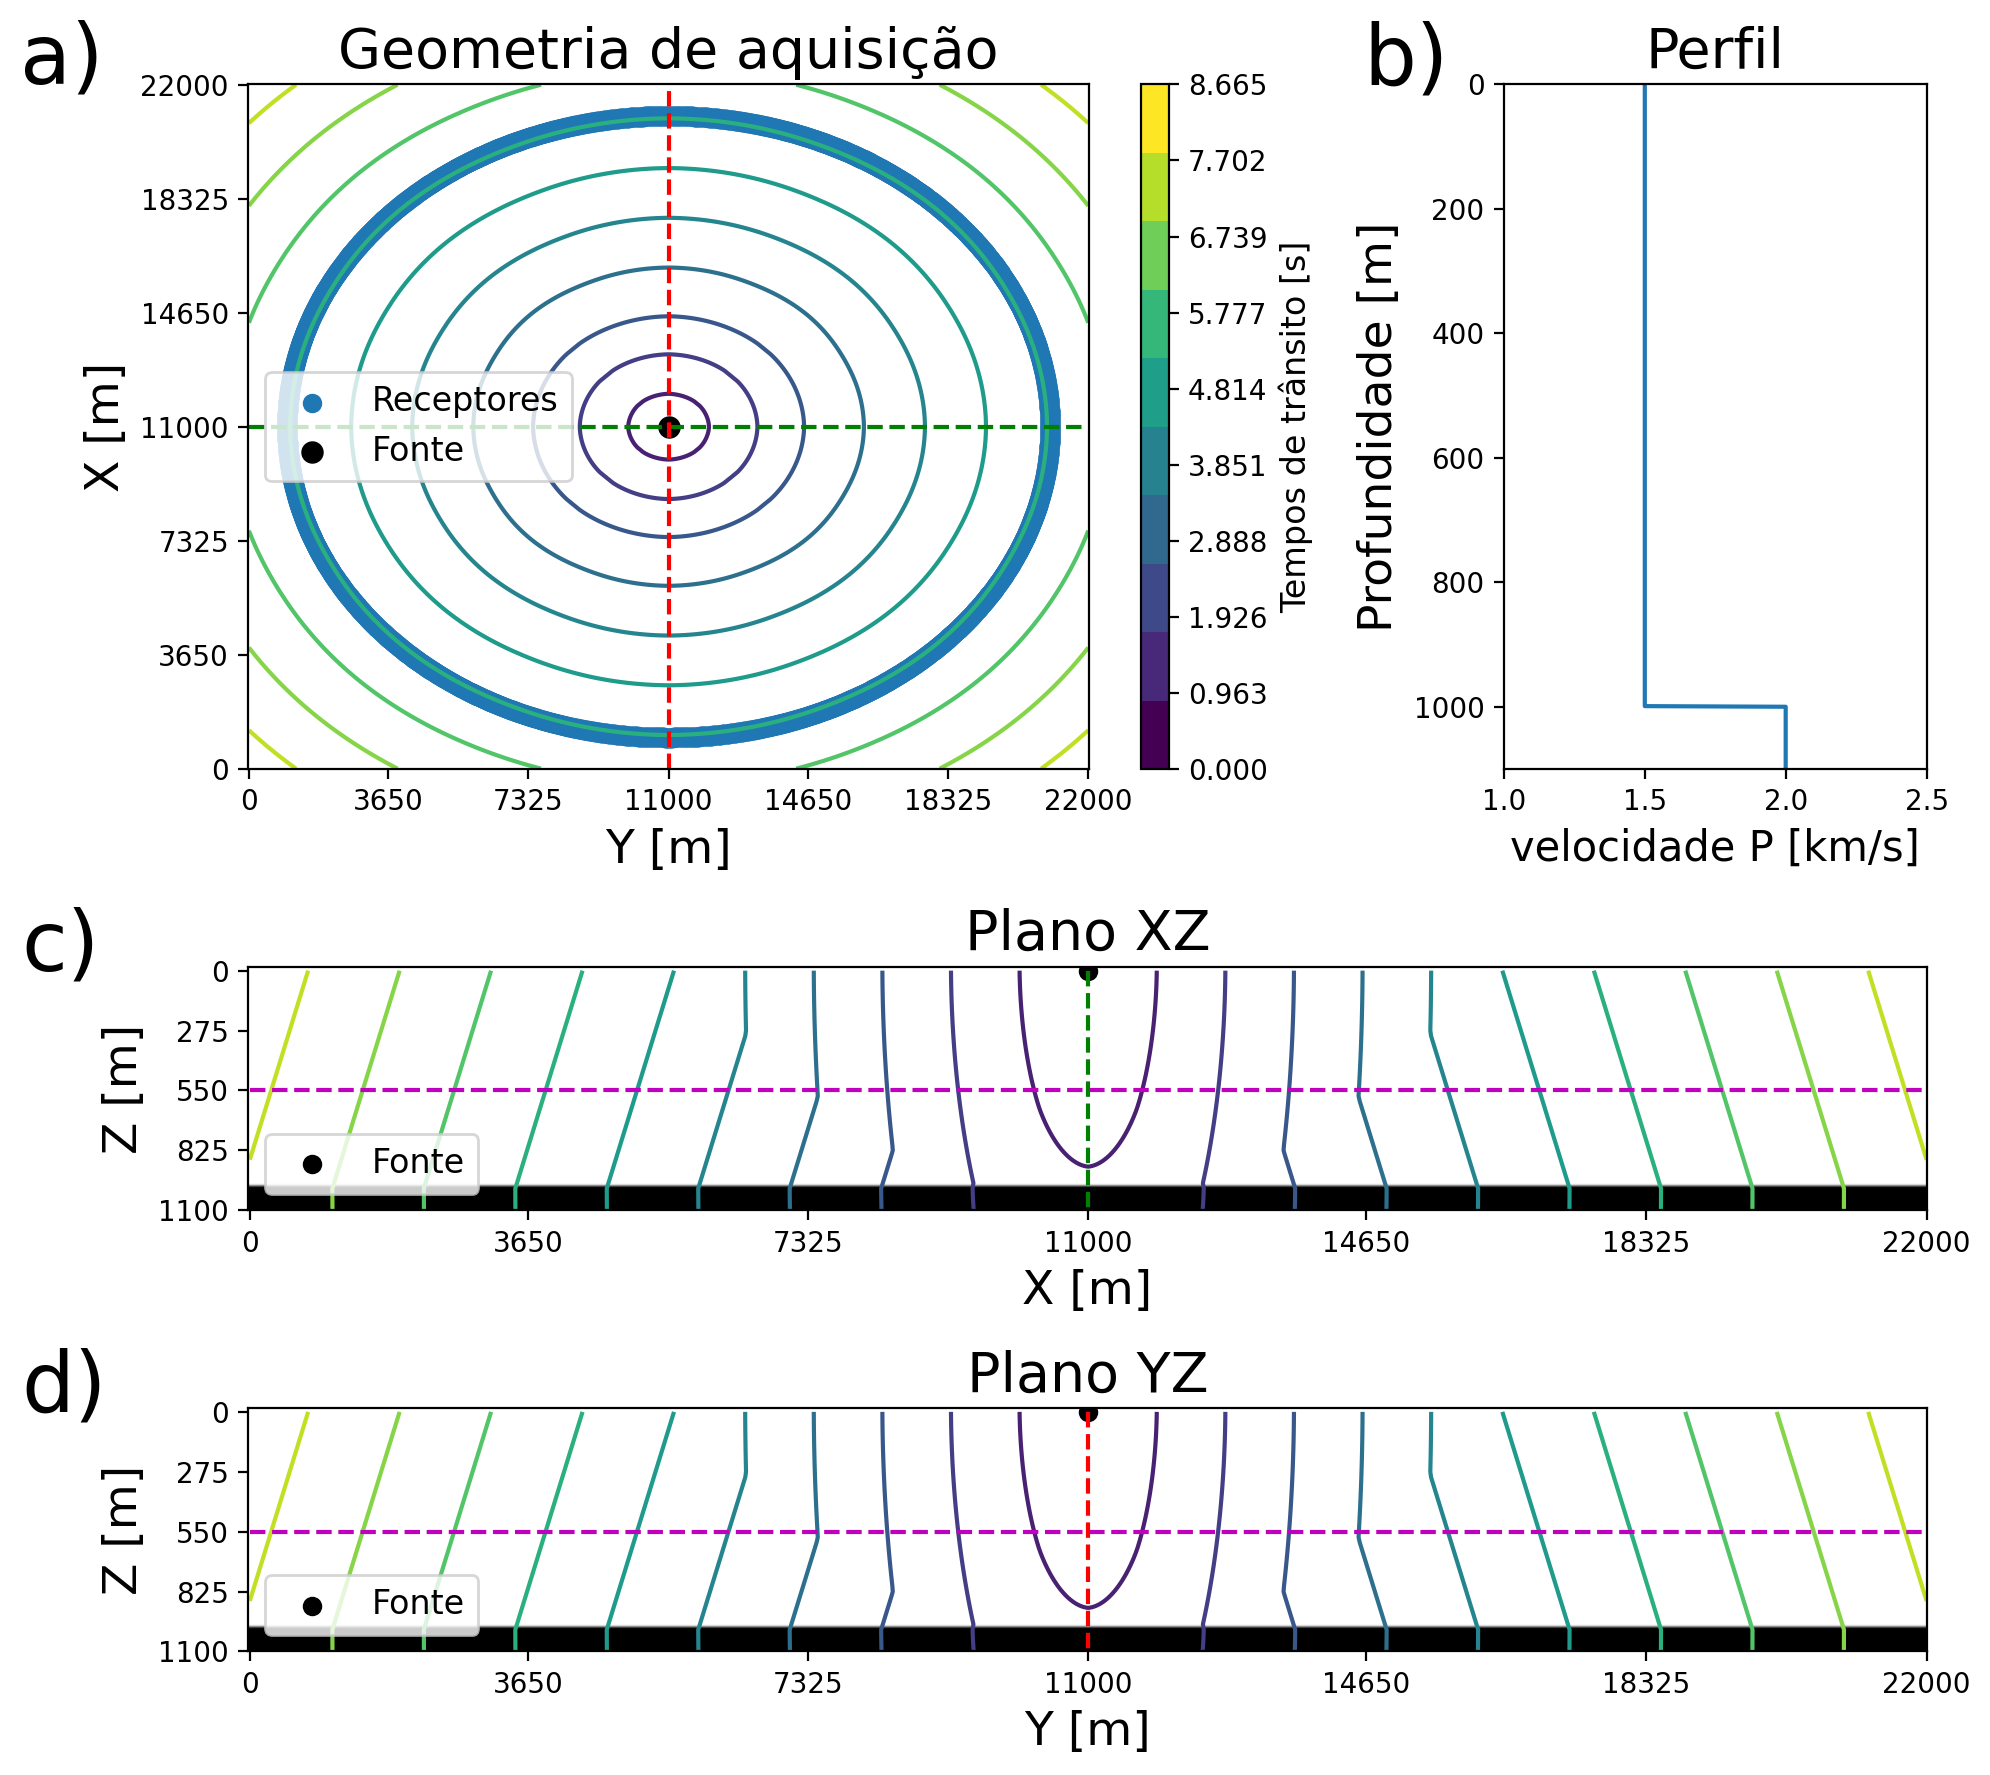
\includegraphics[width = 11cm, height = 10cm]{Imgs/RevisaoBibliografica/modelGeometry.png}
	\caption{Modelo empregado no teste de precisão e performance. (a) Plano XY ilustrando a geometria de aquisição com o arranjo de receptores circulares possuindo somente um tiro central. Isócronas mapeando o comportamento dos tempos de trânsito são mostradas. (b) Perfil de velocidades delimitando a posição da interface. (c) e (d) são as projeções dos cortes em planos XZ e YZ em relação à posição da fonte.}
	\label{fig:configurationNumericalComparison}
\end{figure}

\subsection{Aplicação em modelo complexo}

A fim de validar os algoritmos em um modelo realístico, as formulações estudadas foram aplicadas no modelo SEG/EAGE \textit{Overthrust}, ilustrado na Figura \ref{fig:overthrust}, na intenção de verificar o comportamento das frentes de onda e os tempos de execução perante uma simulação com altos contrastes de velocidade. O modelo possui dimensões de  ($z$, $x$, $y$) = (4.5, 20, 20) km e parâmetro de discretização de 25 m, totalizando (181, 801, 801) amostras. O esquema de geometria circular foi utilizado possuindo três círculos na superfície do modelo com afastamentos 5500, 7500 e 9500 metros do centro do modelo, onde a posição da fonte se encontra. O espaçamento entre os receptores é de 25 m, totalizando 5662 estações, para registrar o máximo de detalhes possível dos tempos gerados pelas formulações que resolvem a equação eikonal. Como o resultado desse experimento, as primeiras chegadas são apresentadas de forma geral e janelas de aproximação no dado mostram os detalhes que o modelo de alto contraste projeta nos dados calculados. Outro resultado são os tempos de execução das formulações de \citeonline{podvin1991finite}, \citeonline{jeong2008fast} e \citeonline{noble2014accurate} após o cálculo do tempo das ondas de primeira chegada. 

\begin{figure}[H]
	\centering
	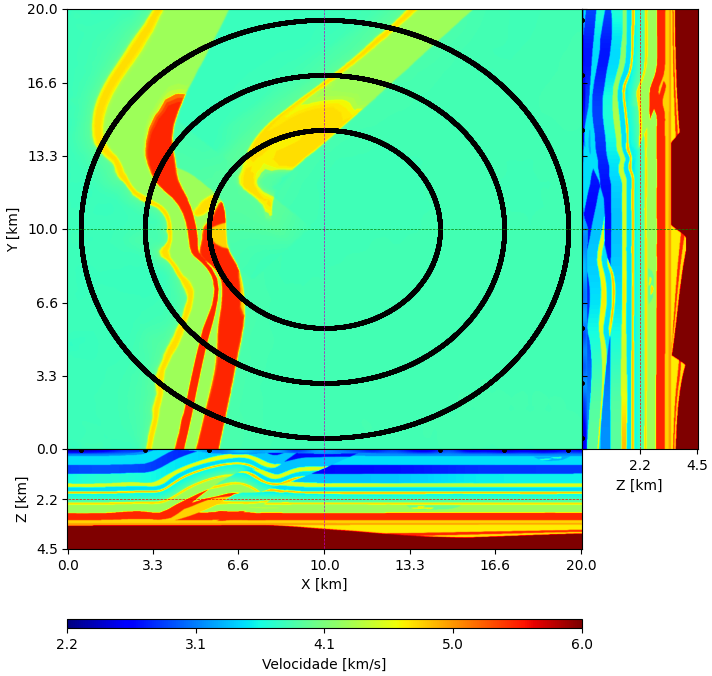
\includegraphics[width = 11cm, height = 10cm]{Imgs/Metodologia/overthrust.png}
	\caption{Modelo SEG/EAGE \textit{Overthrust} para aplicação dos métodos em altos contrastes de velocidade. A geometria circular é aplicada para verificar o comportamento azimutal dos tempos de trânsito. Em preto são os receptores espaçados em 25 metros totalizando 5662 estações. Uma fonte é a plicada no centro do modelo.}
	\label{fig:overthrust}
\end{figure}

\section{Experimento tomográfico}

O experimento realizado parte de um modelo de referência construído por duas superfícies limitantes que ditam a velocidade em cada região. Uma geometria de aquisição baseada em \textit{Ocean Bottom Nodes} é explorada utilizando o princípio da reciprocidade. O modelo inicial é simplesmente um gradiente de velocidade vertical que aumenta com a profundidade. O dado observado foi gerado artificialmente utilizando o modelo de referência onde a equação da onda para meios acústicos de densidade constante foi resolvida. Os dados de primeira chegada foram coletados com a formulação automática de seleção configurada pela equação \ref{automatic_picking}. Os detalhes de cada etapa do experimento serão mostrados a seguir. 

\subsection{Construção dos modelos de velocidade}

Uma superfície de fundo marinho foi criada para detalhar o modelo de referência e também limitar a variação de velocidade em cada região. A superfície apresentada na Figura \ref{fig:water_bottom_surface_gaussian}, foi criada a partir da soma de três funções gaussianas em duas dimensões. A função geradora pode ser formulada da seguinte maneira
\begin{equation}
	g(x,y) = Ae^{-\frac{1}{2}\left( \left(\frac{x - x_c}{\sigma_x}\right)^2 + \left(\frac{y - y_c}{\sigma_y}\right)^2 \right)}   
	\label{gaussian_function}
\end{equation} 
\noindent onde $A$ é a magnitude do pico da função, $\sigma_x$ e $\sigma_y$ são os desvios padrões em cada direção, $x_c$ e $y_c$ são as componentes do centro da gaussiana nas direções $x$ e $y$ respectivamente. A dimensão do plano $xy$ que contemplará todas as superfícies tem dimensões de 7000 x 5000 metros nas direções $x$ e $y$, respectivamente. Para gerar a superfície do fundo marinho três gaussianas foram alocadas fornecendo complexidade à superfície, onde os parâmetros podem ser encontrados na tabela \ref{water_bottom_gaussian_coefs}.  
\begin{table}[H]
	\caption{Lista de coeficientes utilizados para gerar a superfície do fundo marino.}
	\begin{tabular}{c|ccc}
		& $g_1$    & $g_2$  & $g_3$ \\ \hline 
		$A$        & 100 m    & -50 m  & -50 m \\ \hline
		$x_c$      & 100 m    & 5000 m & 5000 m  \\ \hline
		$y_c$      & 2500 m   & 100 m  & 4900 m  \\ \hline
		$\sigma_x$ & 2000 m   & 2000 m & 2000 m  \\ \hline
		$\sigma_y$ & $10^5$ m & 1000 m & 1000 m
	\end{tabular}
	\label{water_bottom_gaussian_coefs}
\end{table}
\noindent Sabendo a superfície do fundo marinho, o modelo de velocidades assumiu a velocidade de 1500 m/s do topo até a base do mar simulado, originando a primeira camada do modelo de referência. 
\begin{figure}[H]
	\centering
	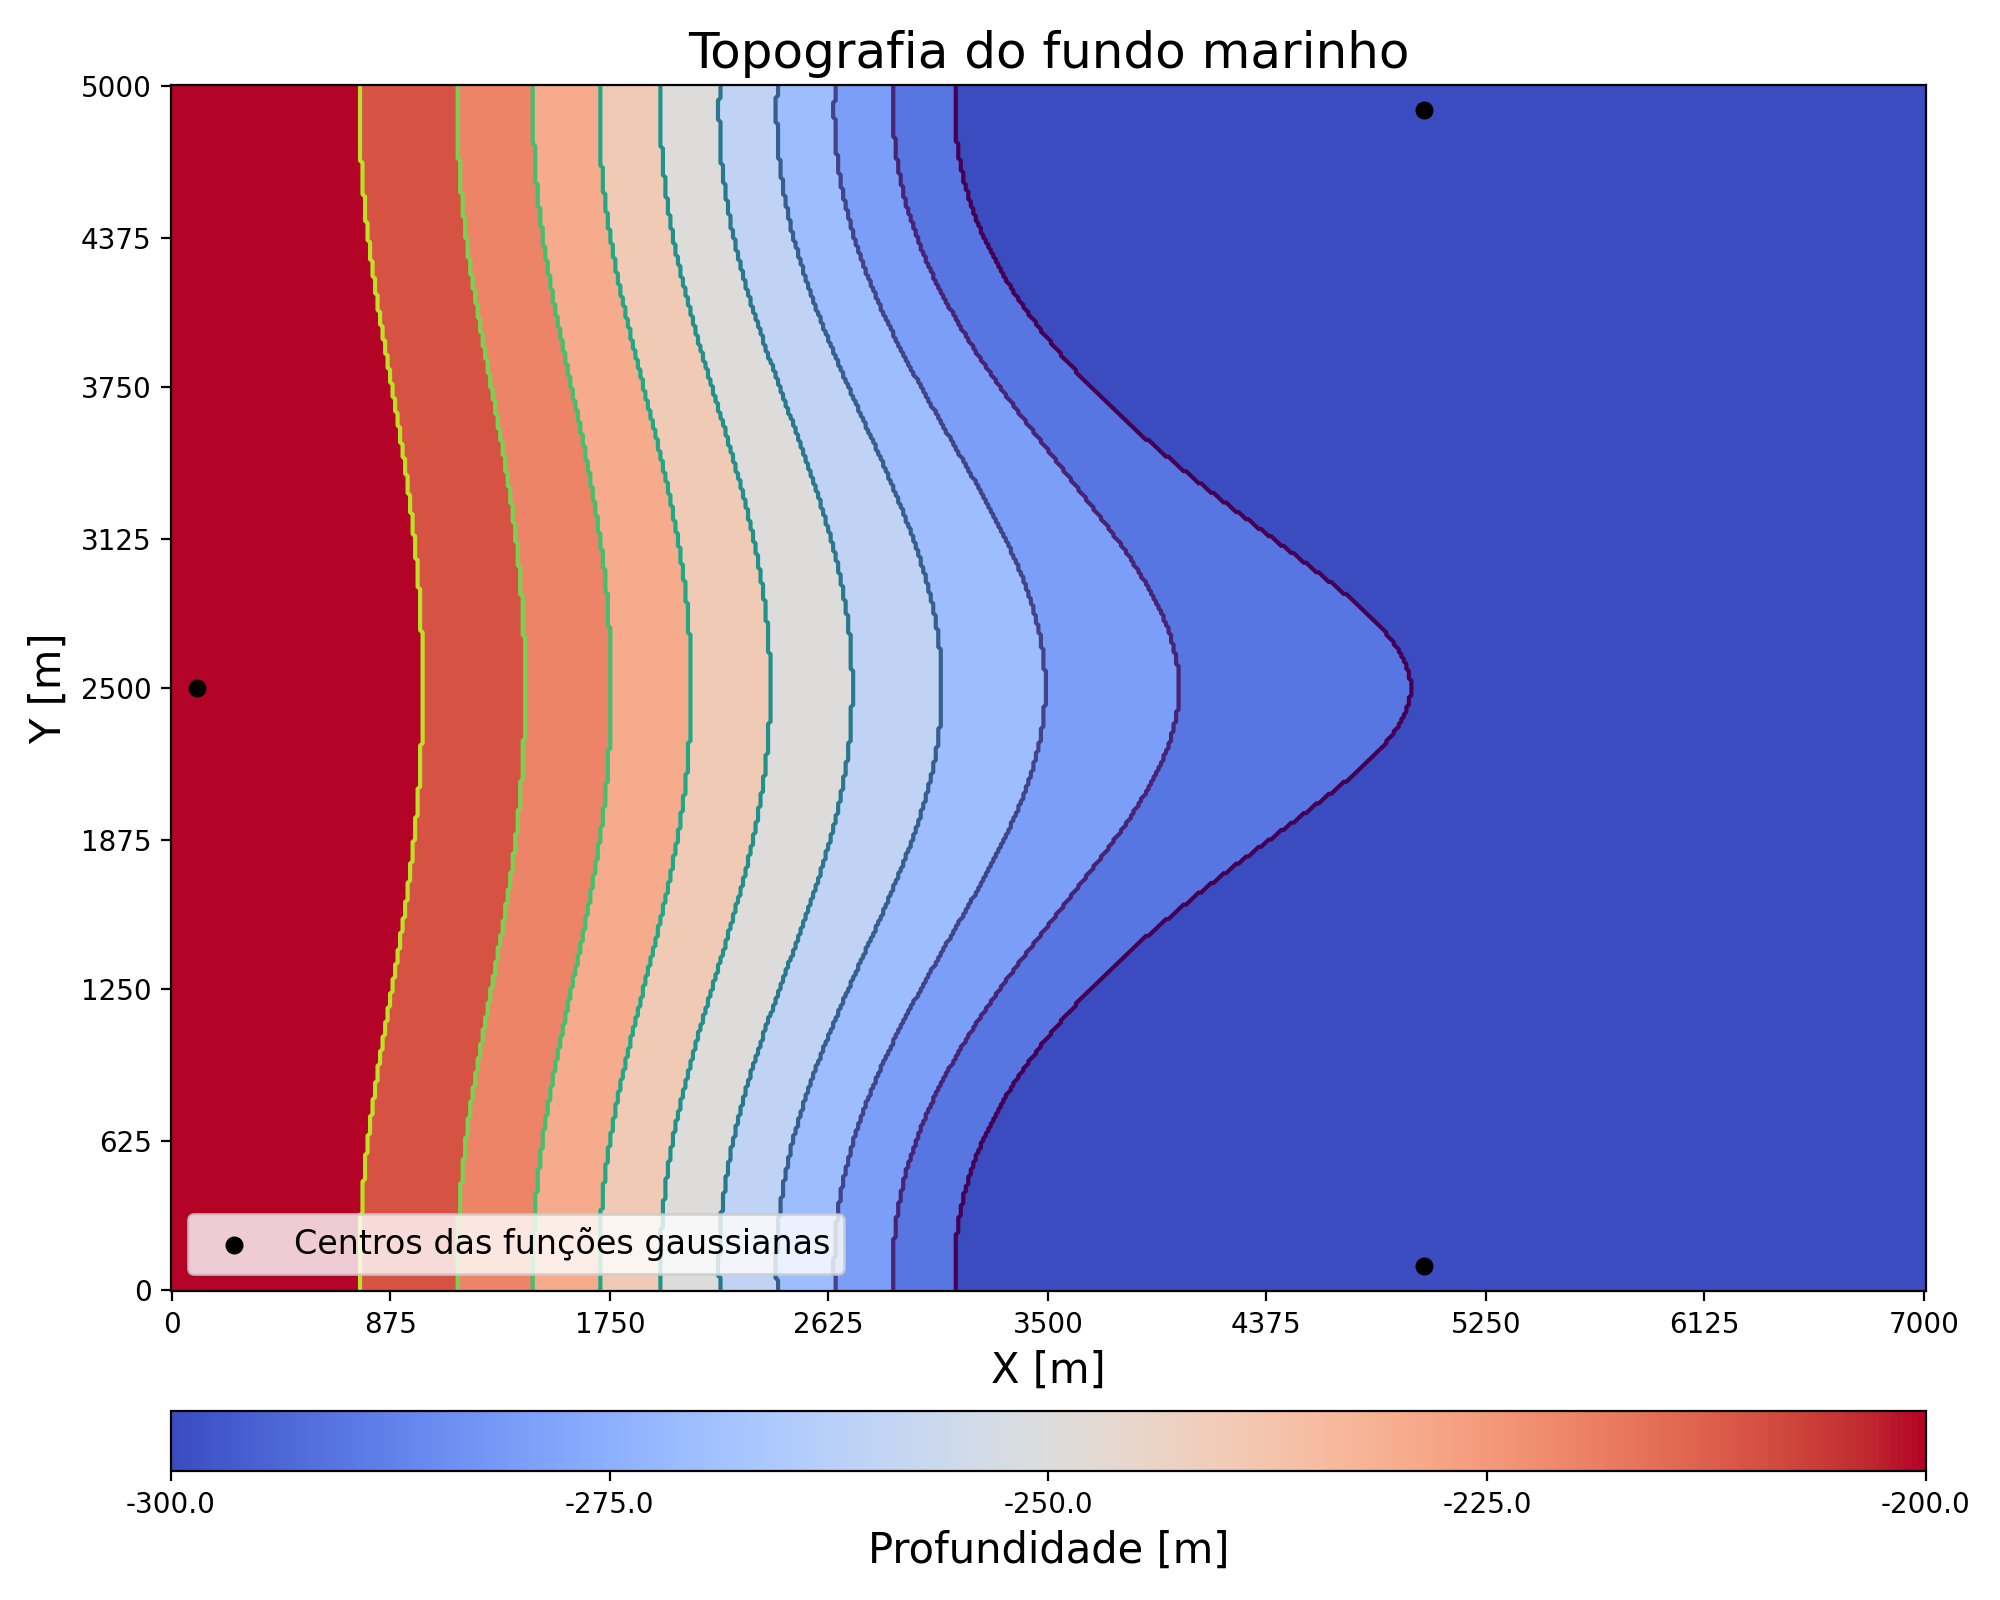
\includegraphics[width=11cm,height=8cm]{Imgs/Metodologia/water_bottom_surface_gaussian.png}
	\caption{Superfície do fundo marinho com o posicionamento dos centros das gaussianas aplicadas. Elevação predominantemente entre 300 e 200 m de profundidade.}
	\label{fig:water_bottom_surface_gaussian}	
\end{figure}
A segunda etapa se concretiza a partir da construção da superfície alvo, sendo formada pela sobreposição de cinco gaussianas formuladas pela equação \ref{gaussian_function}. Os coeficientes para construir a superfície alvo podem ser encontrados na tabela \ref{target_gaussian_coefs}.
\begin{table}[H]
	\caption{Lista de coeficientes utilizados para gerar a superfície alvo.}
	\begin{tabular}{c|ccccc}
		& $g_1$  & $g_2$  & $g_3$  & $g_4$  & $g_5$  \\ \hline
		$A$        & 550 m  & 600 m  & -300 m & 450 m  & 400 m  \\ \hline
		$x_c$      & 2500 m & 2500 m & 3500 m & 4500 m & 4500 m \\ \hline
		$y_c$      & 2000 m & 3000 m & 2500 m & 2000 m & 3000 m \\ \hline
		$\sigma_x$ & 800 m  & 800 m  & 500 m  & 800 m  & 800 m  \\ \hline
		$\sigma_y$ & 500 m  & 500 m  & 300 m  & 600 m  & 600 m 
	\end{tabular}
	\label{target_gaussian_coefs}
\end{table}
\noindent A partir da superfície ilustrada na Figura \ref{fig:target_surface_gaussian}, um gradiente de velocidade crescente com a profundidade foi aplicado seguindo a equação 
\begin{equation}
	v(z) = 1650 + 100 z,
\end{equation}
\noindent onde a velocidade $v$ aumenta 100 m/s por metro, iniciando em 1650 m/s, entre o limite do fundo marinho e a superfície alvo. Para completar o modelo de velocidade de referência, abaixo da superfície alvo o valor de 3500 m/s foi atribuído até a profundidade de 1000 metros construindo o modelo mostrado na Figura \ref{fig:true_model}.
\begin{figure}[H]
	\centering
	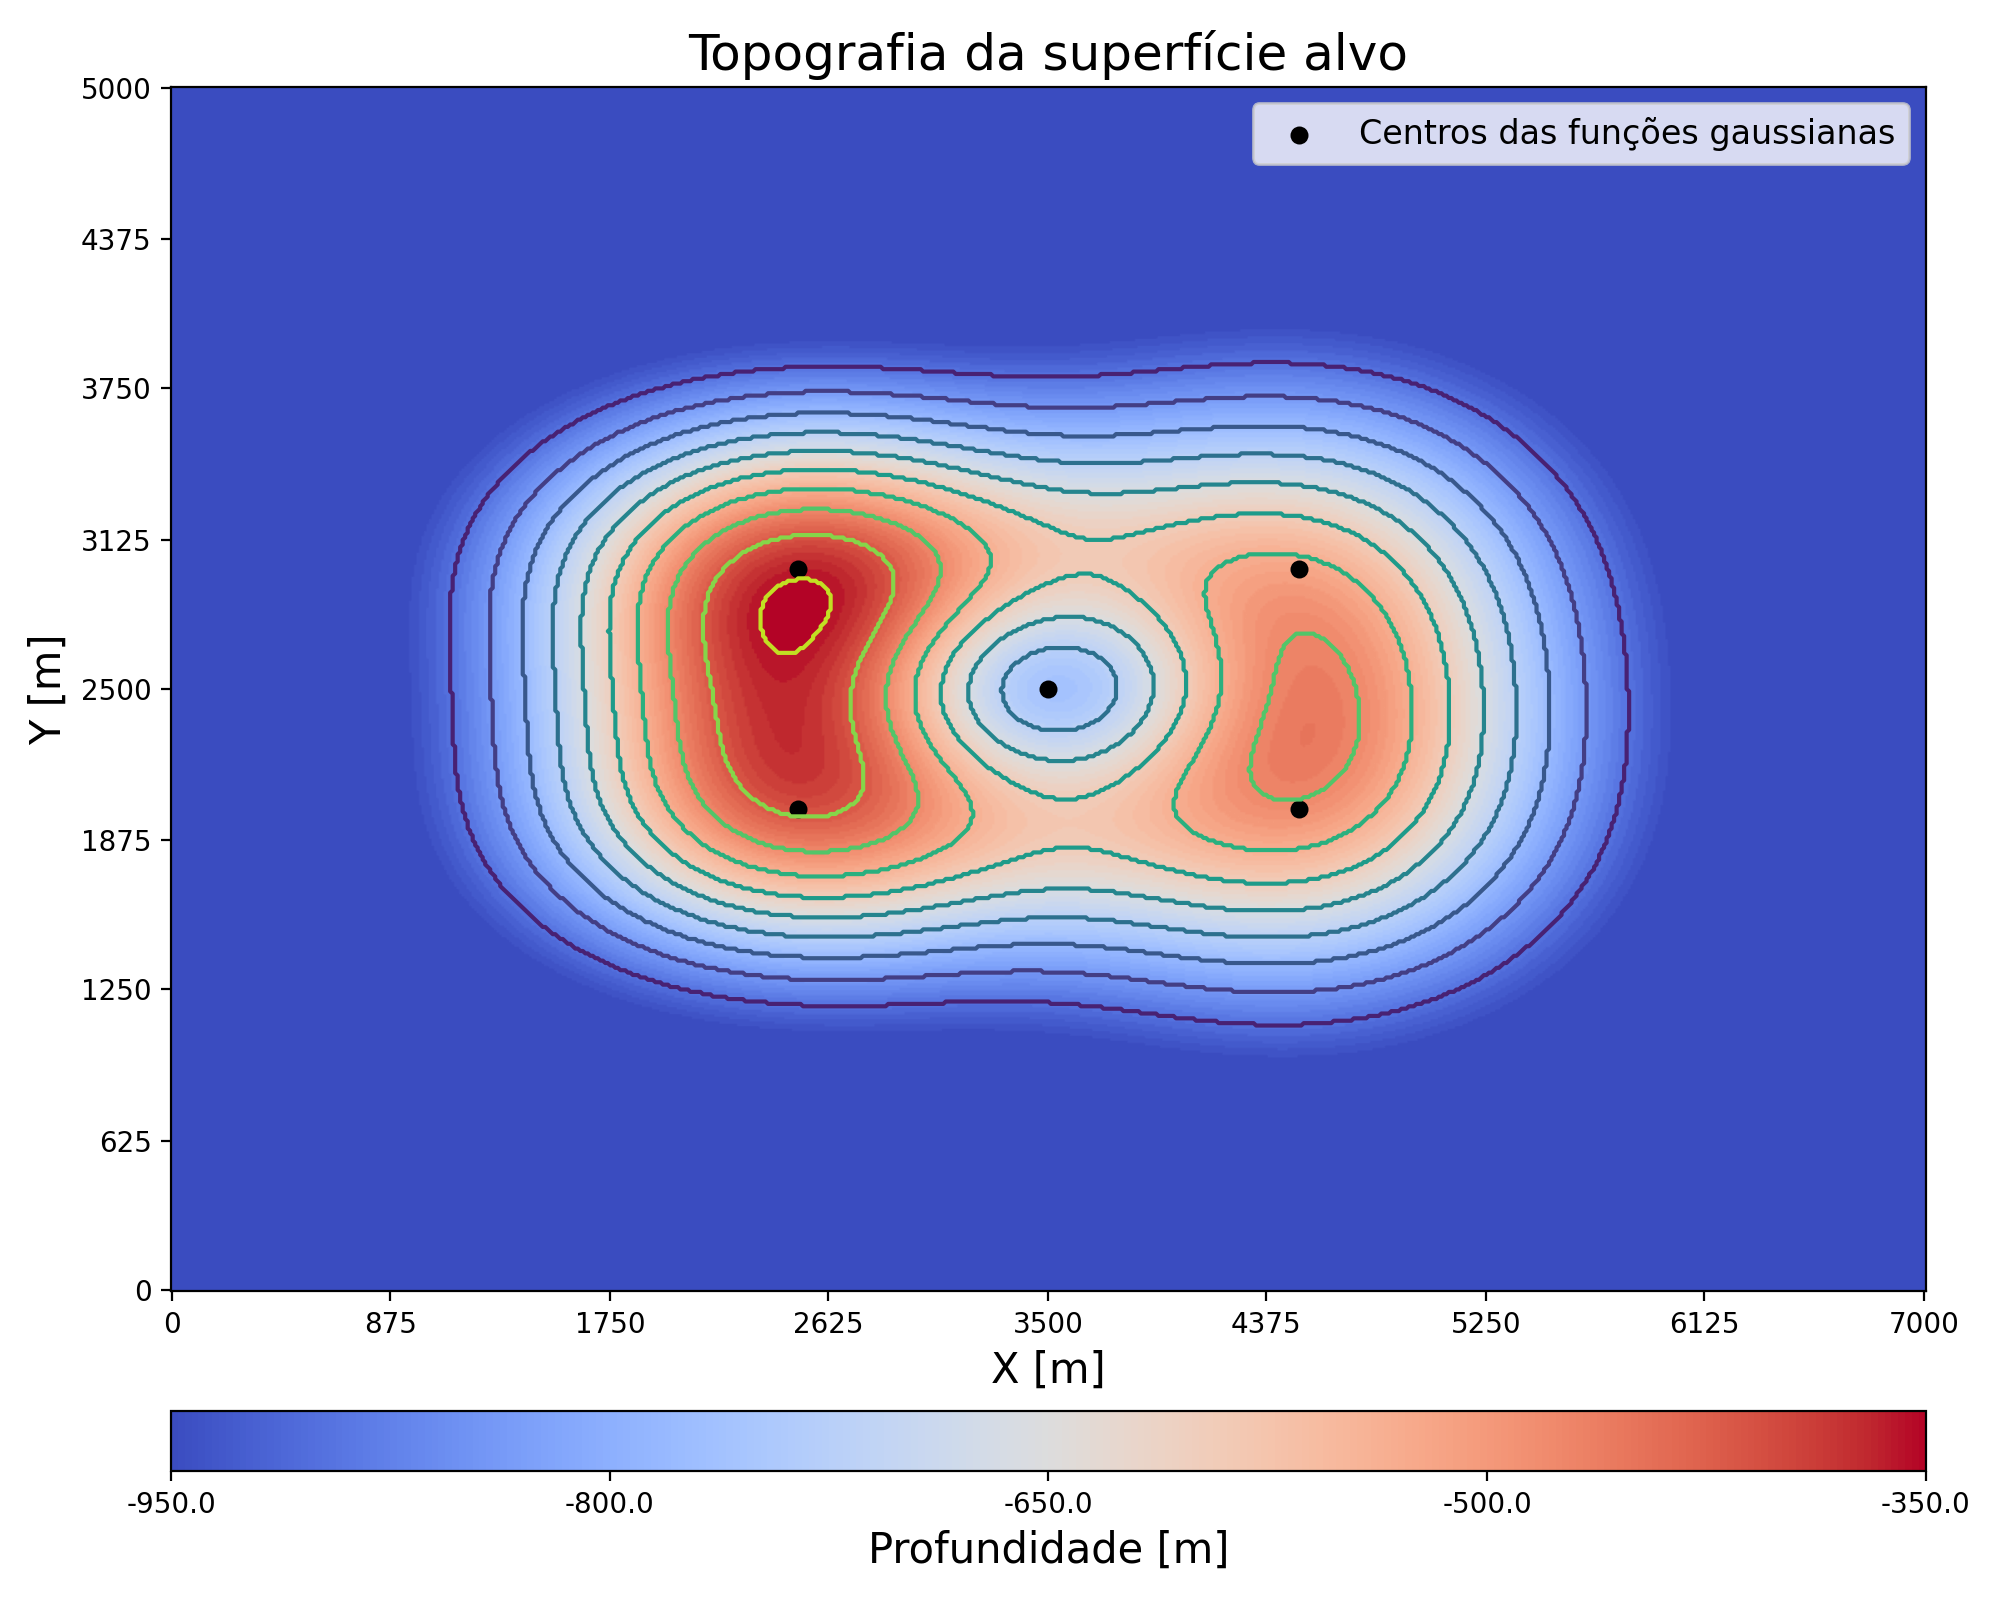
\includegraphics[width=11cm,height=8cm]{Imgs/Metodologia/target_surface_gaussian.png}
	\caption{Superfície alvo com o posicionamento dos centros das gaussianas aplicadas. Elevação entre 950 e 350 m de profundidade.}
	\label{fig:target_surface_gaussian}	
\end{figure}
O modelo inicial, ilustrado na Figura \ref{fig:init_model}, foi construído com base na formulação $v(z) = 1650 + 250z$, onde o aumento de velocidade varia em 250 m/s por metro, partindo de uma profundidade fixa de 250 m definida como base do fundo marinho hipotético.  
\begin{figure}[H]
	\centering
	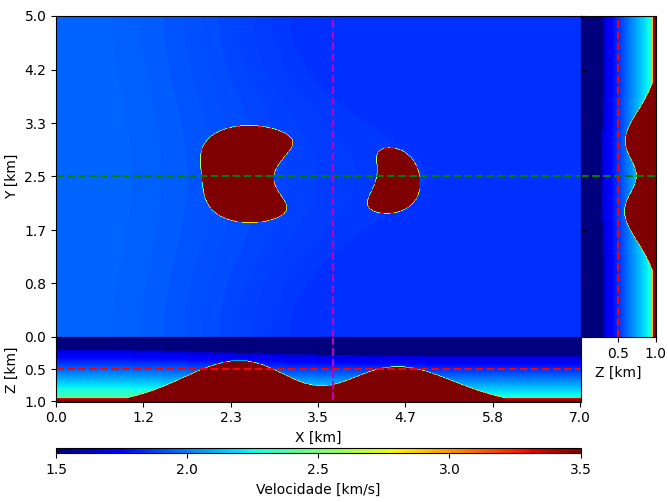
\includegraphics[width=12cm,height=9cm]{Imgs/Metodologia/true_model.png}
	\caption{Modelo de referência para gerar o dado observado. Variação de velocidade entre 1500 e 3500 m/s. Tentativa de simulação com altos contrastes de velocidade.}
	\label{fig:true_model}	
\end{figure}
Acima do horizonte plano hipotético, a velocidade no modelo inicial recebe 1500 m/s e varia até a mesma grandeza do modelo de referência, 350 m/s. A variação em forma de gradiente simula camadas planas sem velocidades variando lateralmente, processo comum para inicializar problemas tomográficos em regiões ainda desconhecidas. 
\begin{figure}[H]
	\centering
	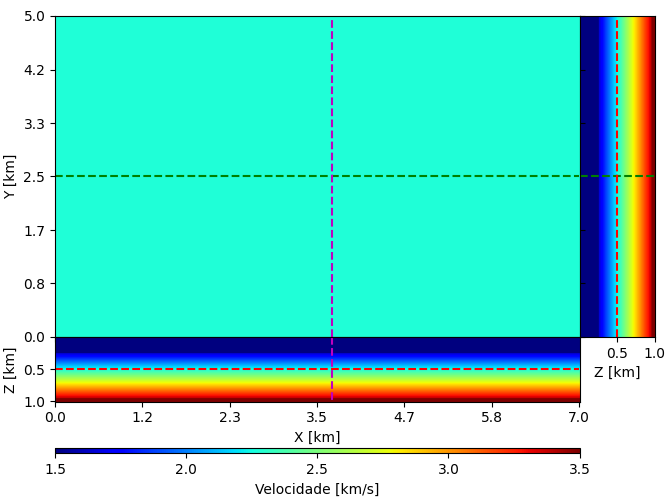
\includegraphics[width=12cm,height=9cm]{Imgs/Metodologia/init_model.png}
	\caption{Modelo base para inicializar o processo tomográfico. Simulação de camadas plano paralelas com baixos contrastes de velocidade seguindo uma equação de gradiente linear com a profundidade.}
	\label{fig:init_model}	
\end{figure}

\subsection{Geometria de aquisição}

Tanto para registrar o dado observado no modelo de referência quanto para recuperar as variações do modelo em relação aos dados, a mesma geometria de aquisição foi utilizada. A composição do arranjo de fontes tem dimensões de 140 e 100 unidades nas direções $x$ e $y$, respectivamente. As fontes se encontram na mesma profundidade de 10 metros e no total formam 14000 unidades. Os receptores estão posicionados no fundo marinho seguindo a projeção da superfície ilustrada na Figura \ref{fig:water_bottom_surface_gaussian}. Totalizando 176 unidades, suas componentes se separam entre 16 e 11 unidades nas direções $x$ e $y$, respectivamente. Pela densidade de tiros aplicados na superfície do mar, o princípio da reciprocidade foi utilizado para gerar o dado observado e também para performar a inversão tomográfica, onde as fontes assumem a função dos receptores e vice-versa. A Figura \ref{fig:complete_geometry} exibe a densidade das fontes em relação aos receptores na aquisição simulada. A Figura \ref{fig:true_model_geometry} mostra a geometria projetada no modelo de referência, ilustrando a variação das posições dos receptores OBN no horizonte do fundo marinho. A Figura \ref{fig:init_model_geometry} ilustra a projeção da geometria no modelo inicial da inversão tomográfica, evidenciando os aspectos planares do horizonte do fundo marinho hipotético. Com a geometria definida, a modelagem de propagação de ondas pode ser efetuada gerando assim o dado observado sintético e os detalhes da criação e seleção do dado estão na próxima seção. 
\begin{figure}[H]
	\centering
	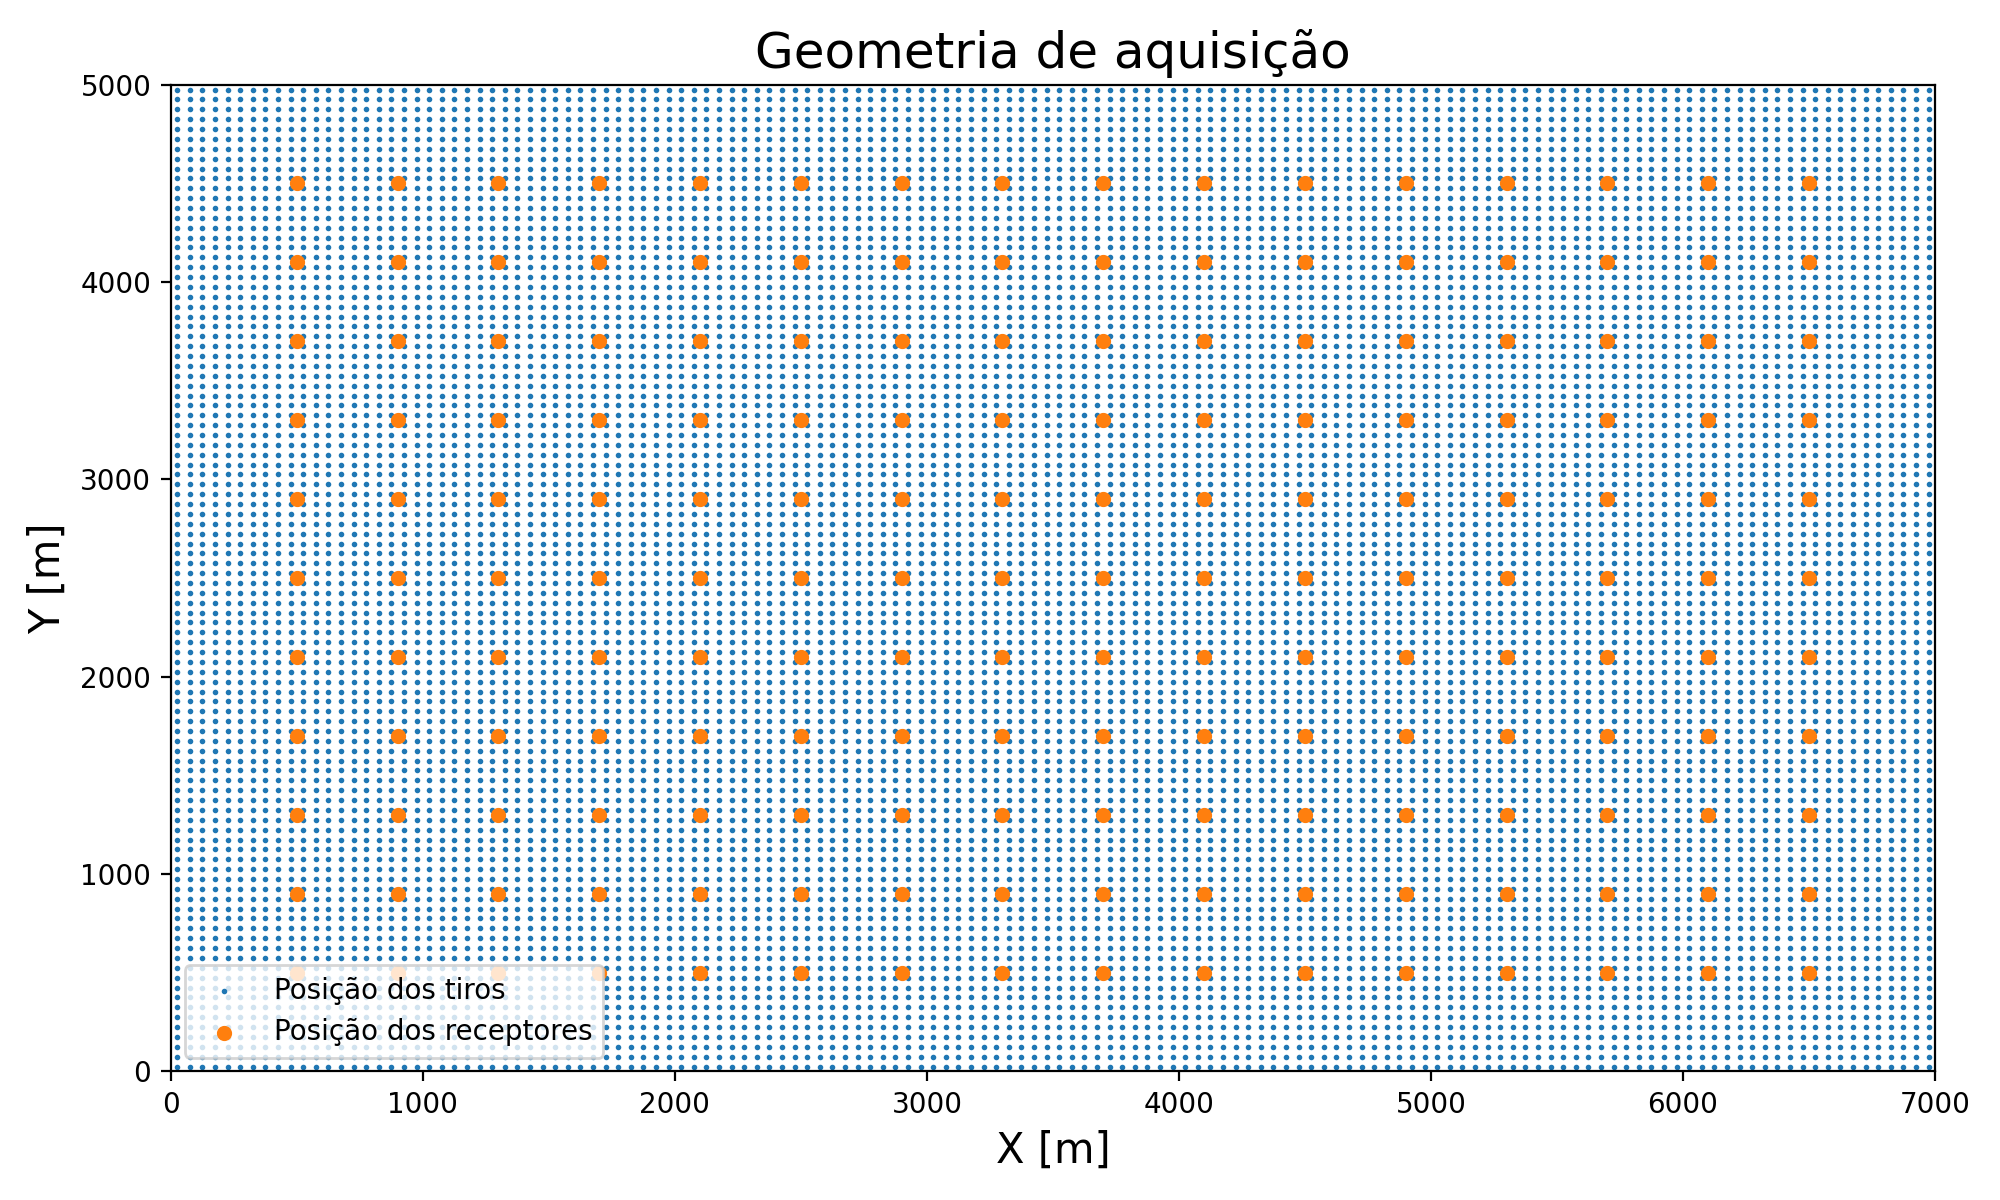
\includegraphics[width=12cm,height=7cm]{Imgs/Metodologia/complete_geometry.png}
	\caption{Configuração da geometria completa de aquisição contendo 176 receptores localizados no fundo marinho e 14000 tiros na superfície do oceano. Foi considerado 50 m para o espaçamento entre tiros e 400 metros para os receptores em ambas direções X e Y.}
	\label{fig:complete_geometry}	
\end{figure}
\begin{figure}[H]
	\centering
	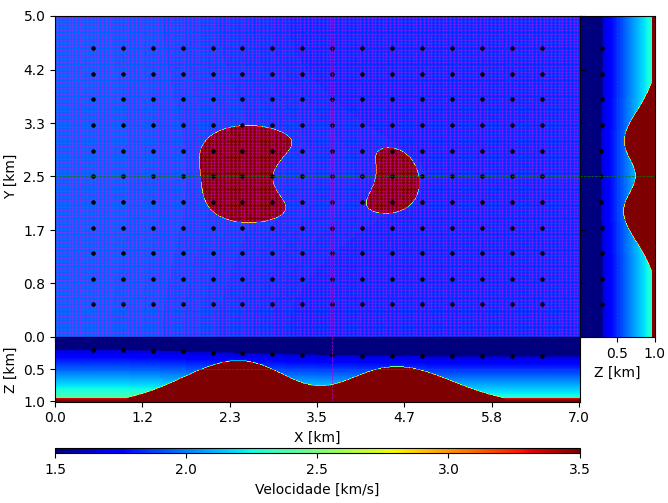
\includegraphics[width=12cm,height=9cm]{Imgs/Metodologia/true_model_geometry.png}
	\caption{Geometria de aquisição projetada no modelo de referência.}
	\label{fig:true_model_geometry}	
\end{figure}
\begin{figure}[H]
	\centering
	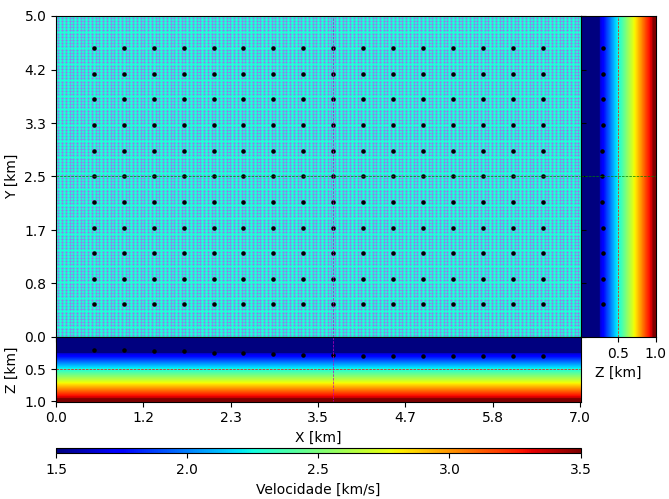
\includegraphics[width=12cm,height=9cm]{Imgs/Metodologia/init_model_geometry.png}
	\caption{Geometria de aquisição projetada no modelo inicial.}
	\label{fig:init_model_geometry}	
\end{figure}

\subsection{Dado observado sintético}

Pensando em utilizar a formulação de primeira chegada automática, onde a energia da onda é alvo dos cálculos, foi levado em consideração a mudança de fase da assinatura da fonte sísmica. A Ricker (equação \ref{ricker}) é uma fonte de fase zero, ou seja, a fonte está definida em tempos positivos e negativos. Na natureza os tempos negativos não são levados em consideração pois o sinal causal deflagrado por uma fonte artificial real começa a ser definido a partir do instante de tempo zero. Utilizando a função Ricker de fase zero, o tempo recuperado pelo método de seleção da primeira chegada não foi satisfatório. Então, uma solução é transformar um pulso de fase zero em um pulso de fase mínima, para que o algoritmo de seleção automática da primeira chegada desenvolvesse seu papel mais precisamente.

A Figura \ref{fig:ricker_zero_phase} mostra os aspectos da fonte Ricker de fase zero. O diagrama de polos e zeros tem papel crucial na transformação do pulso para a fase mínima. Um sinal causal, que têm transformada de Fourier, possui sua região de convergência maior igual ao círculo unitário no domínio complexo \cite{proakis1975digital, oppenheim1987digital, oppenheim1997signals}. Sendo assim, a transformação efetuada foi a multiplicação de cada posição de polo e zero pelo inverso da distância dos mesmos até a origem, gerando uma distância resultante menor que 1 para cada componente do diagrama de polos e zeros. A Figura \ref{fig:ricker_min_phase} mostra a função Ricker após a transformação, sendo que a Figura \ref{fig:ricker_min_phase}b exibe o diagrama de polos e zeros com todos os componentes no interior do círculo unitário.    

\begin{figure}[H]
	\centering
	\subfloat[]{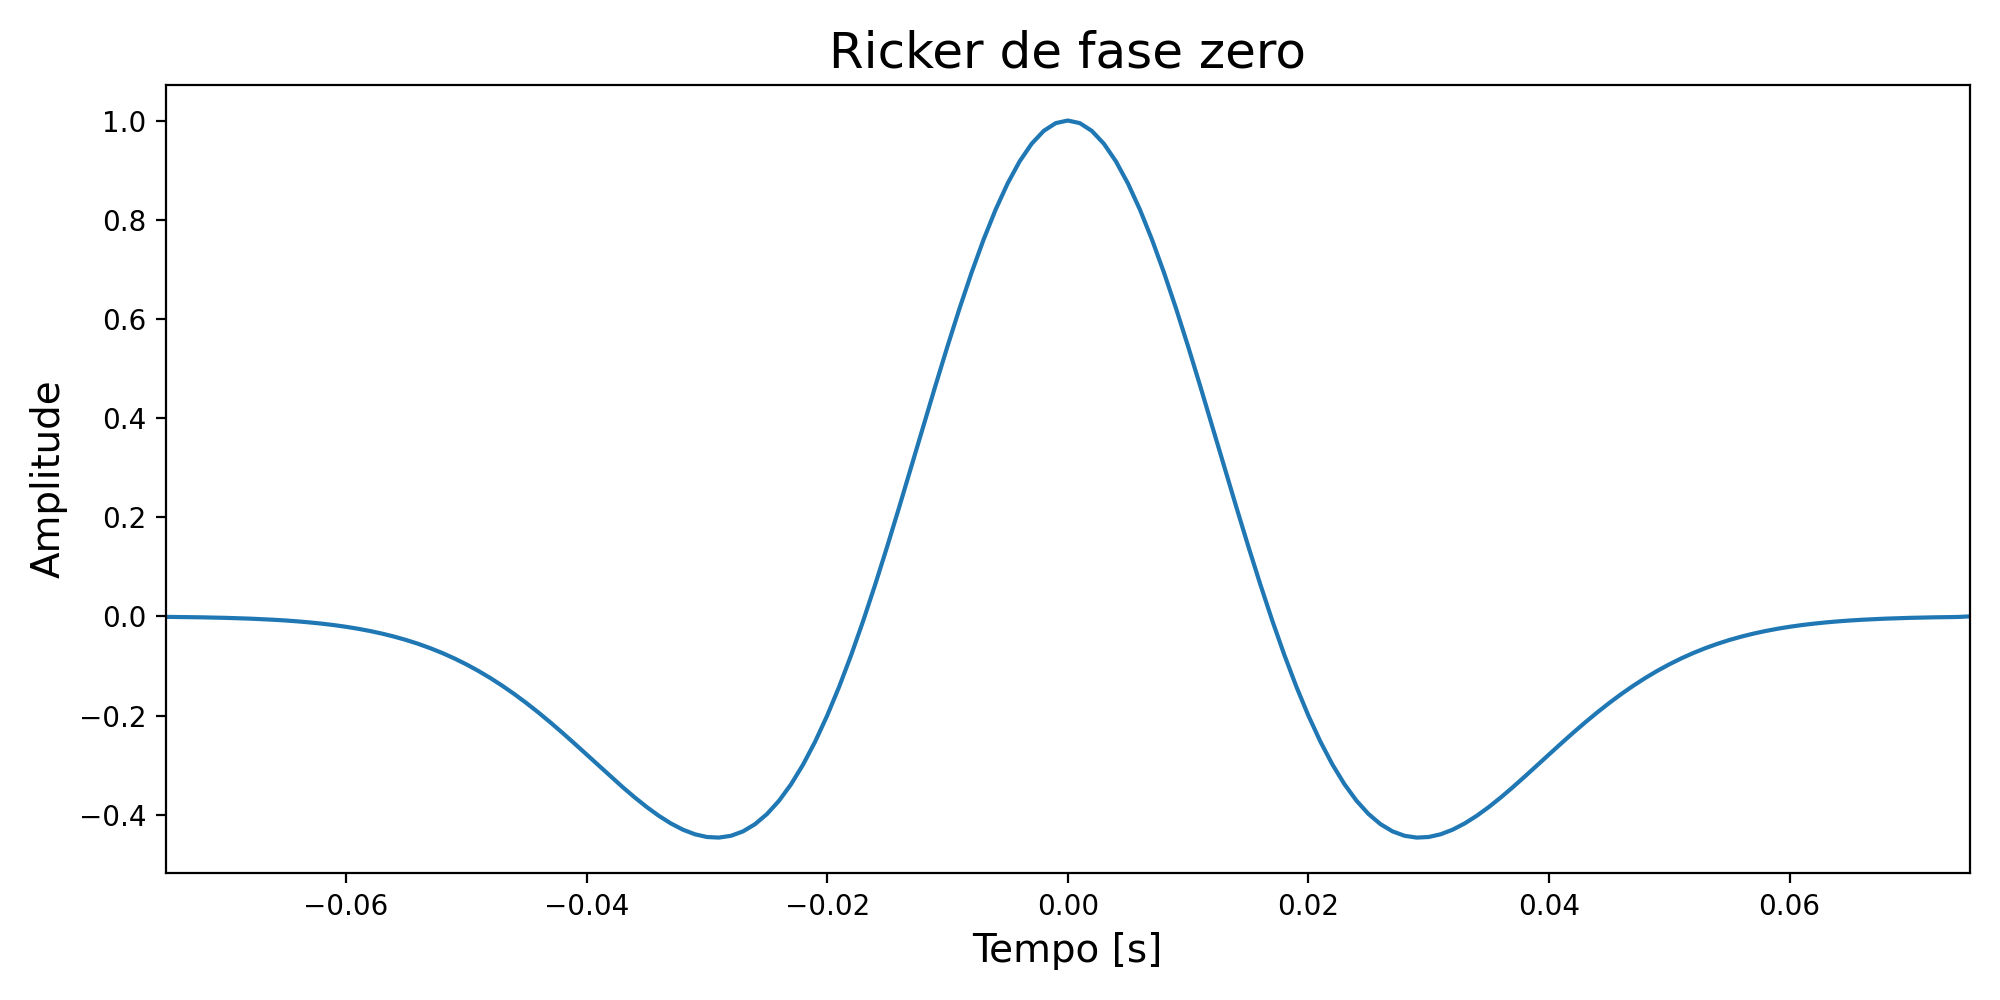
\includegraphics[width=8cm,height=4cm]{Imgs/Metodologia/ricker_zero_phase_a.png}}
	\subfloat[]{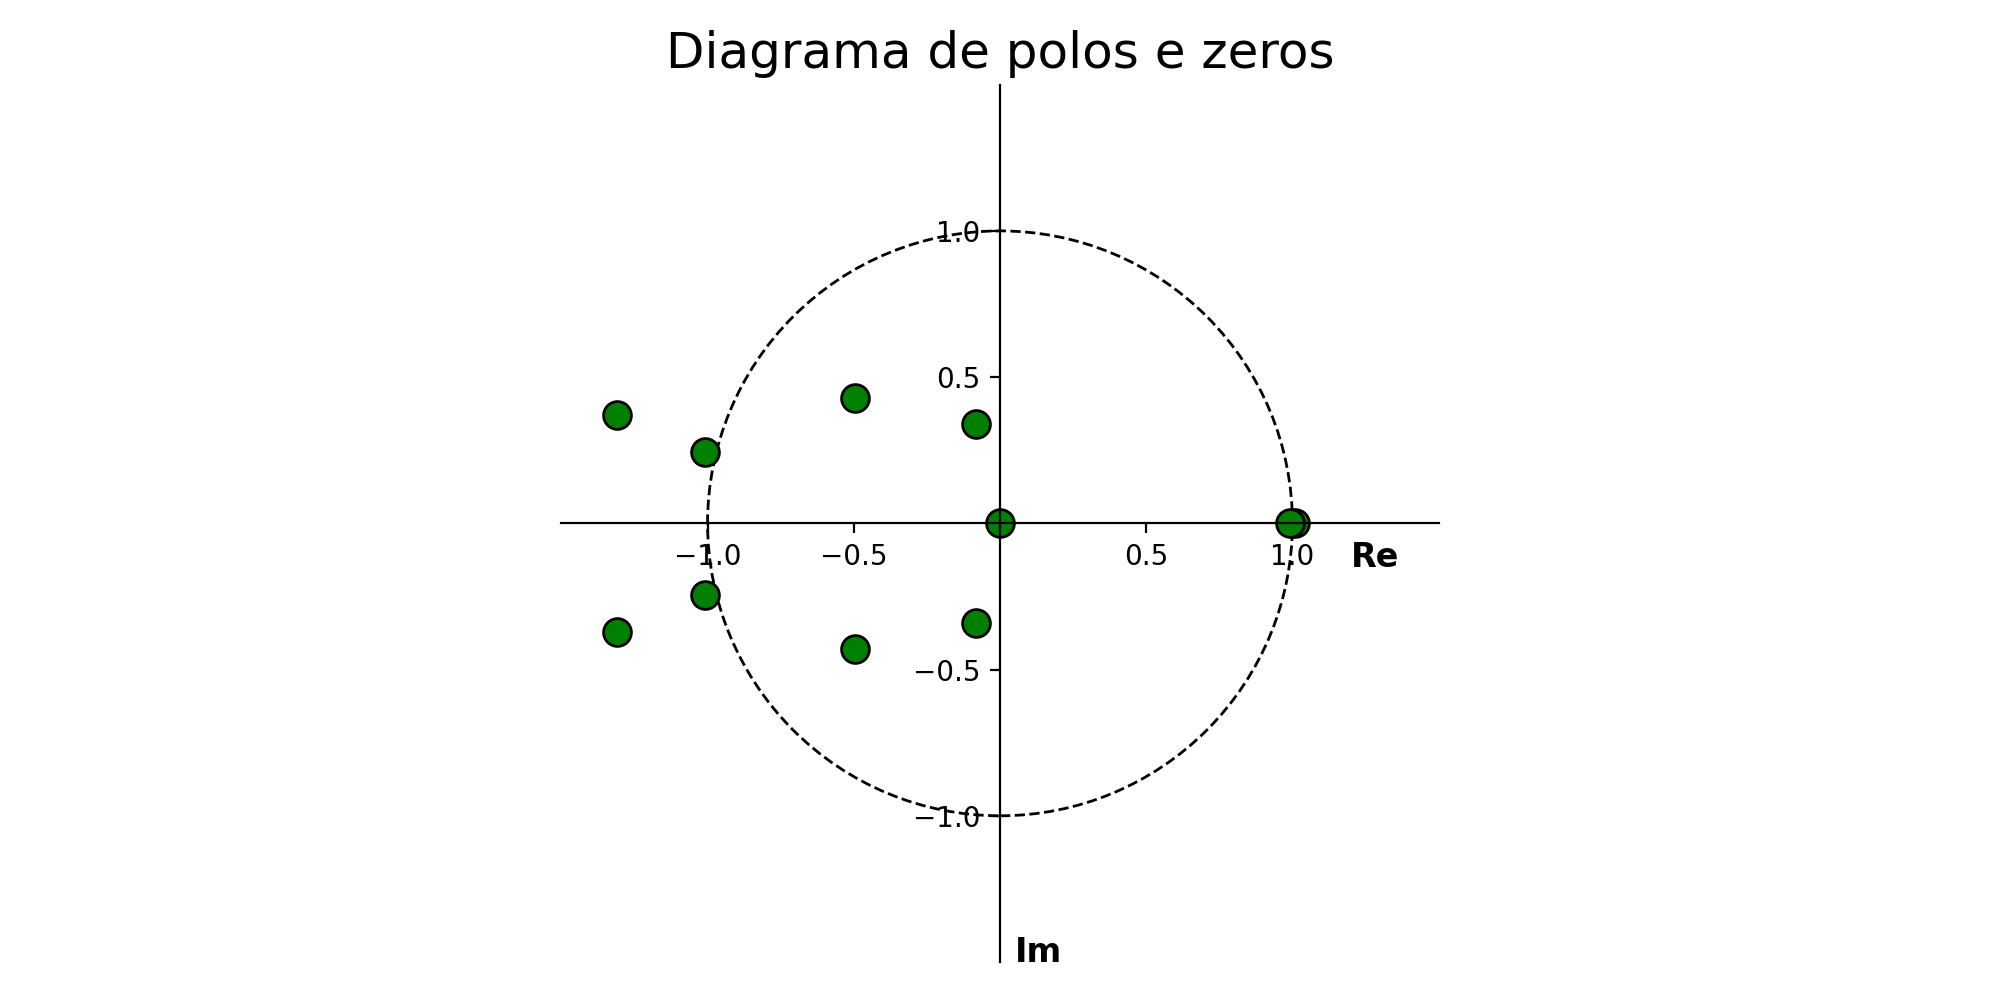
\includegraphics[width=8cm,height=4cm]{Imgs/Metodologia/ricker_zero_phase_b.png}}
	
	\subfloat[]{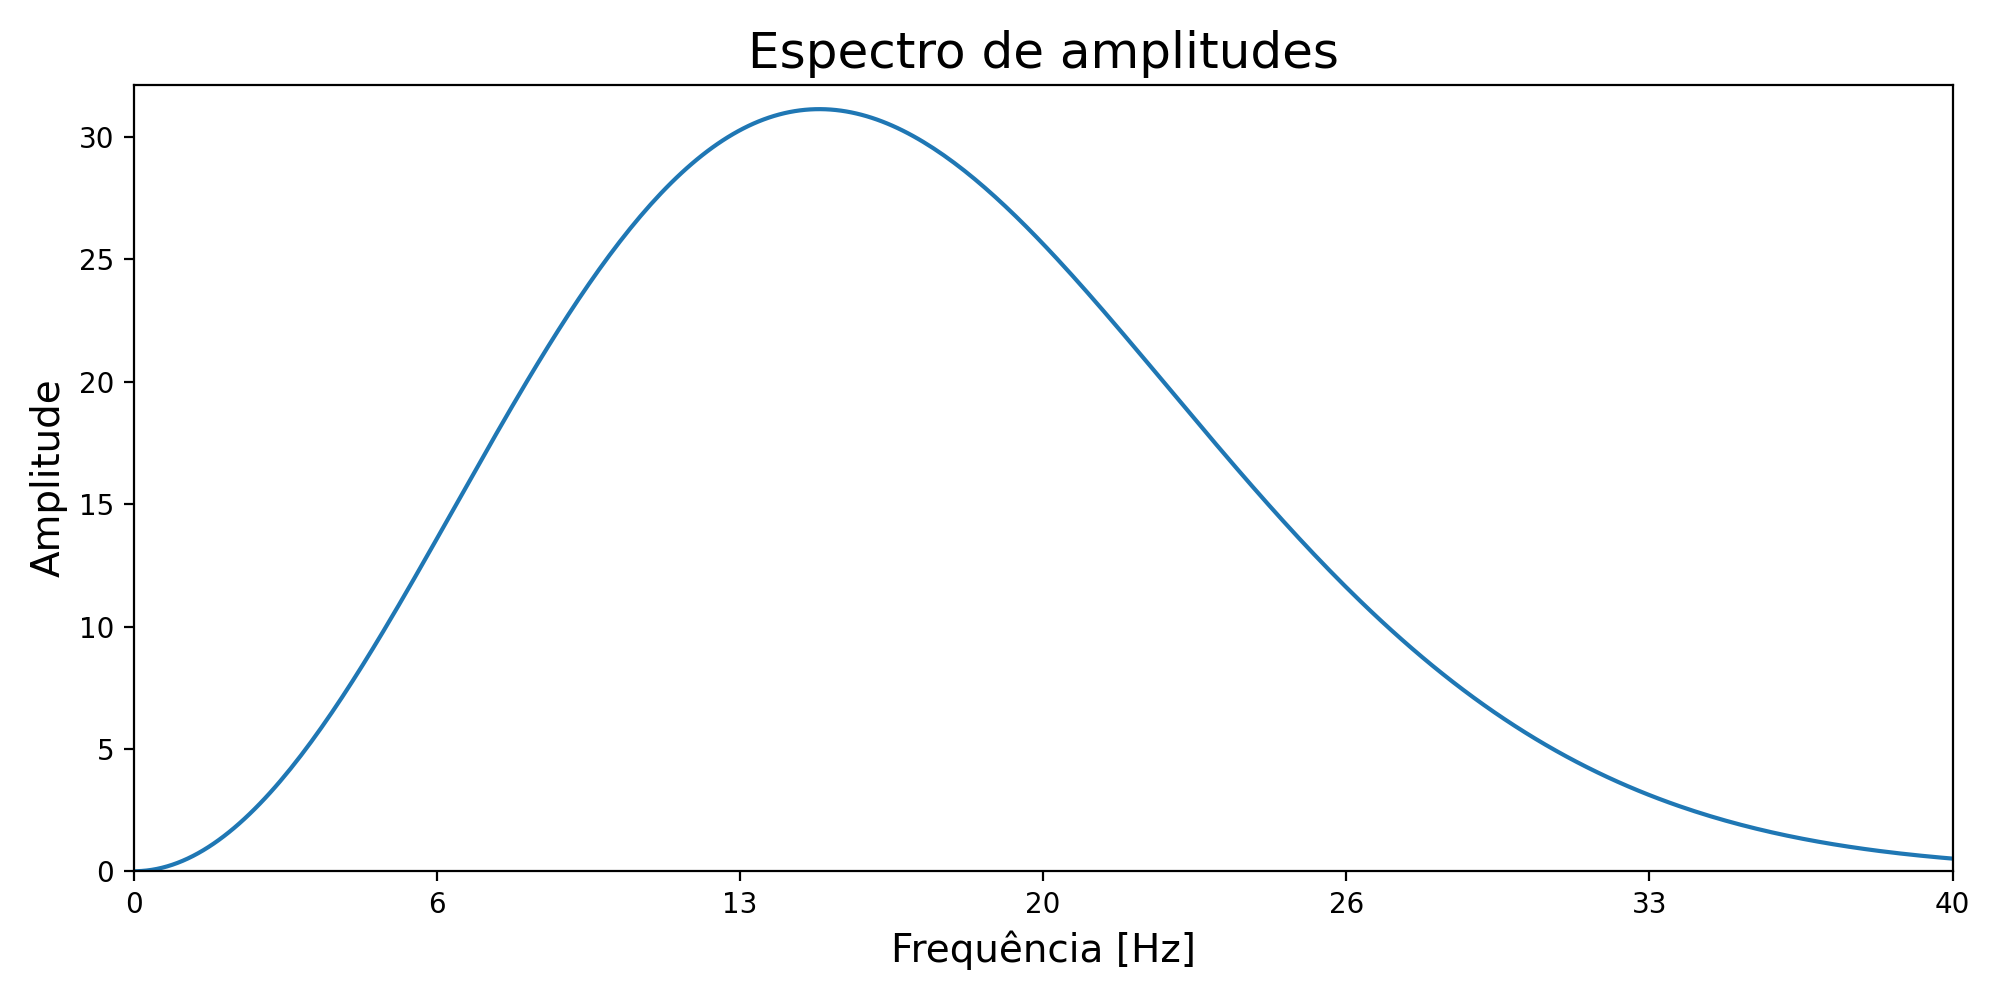
\includegraphics[width=8cm,height=4cm]{Imgs/Metodologia/ricker_zero_phase_c.png}}
	\subfloat[]{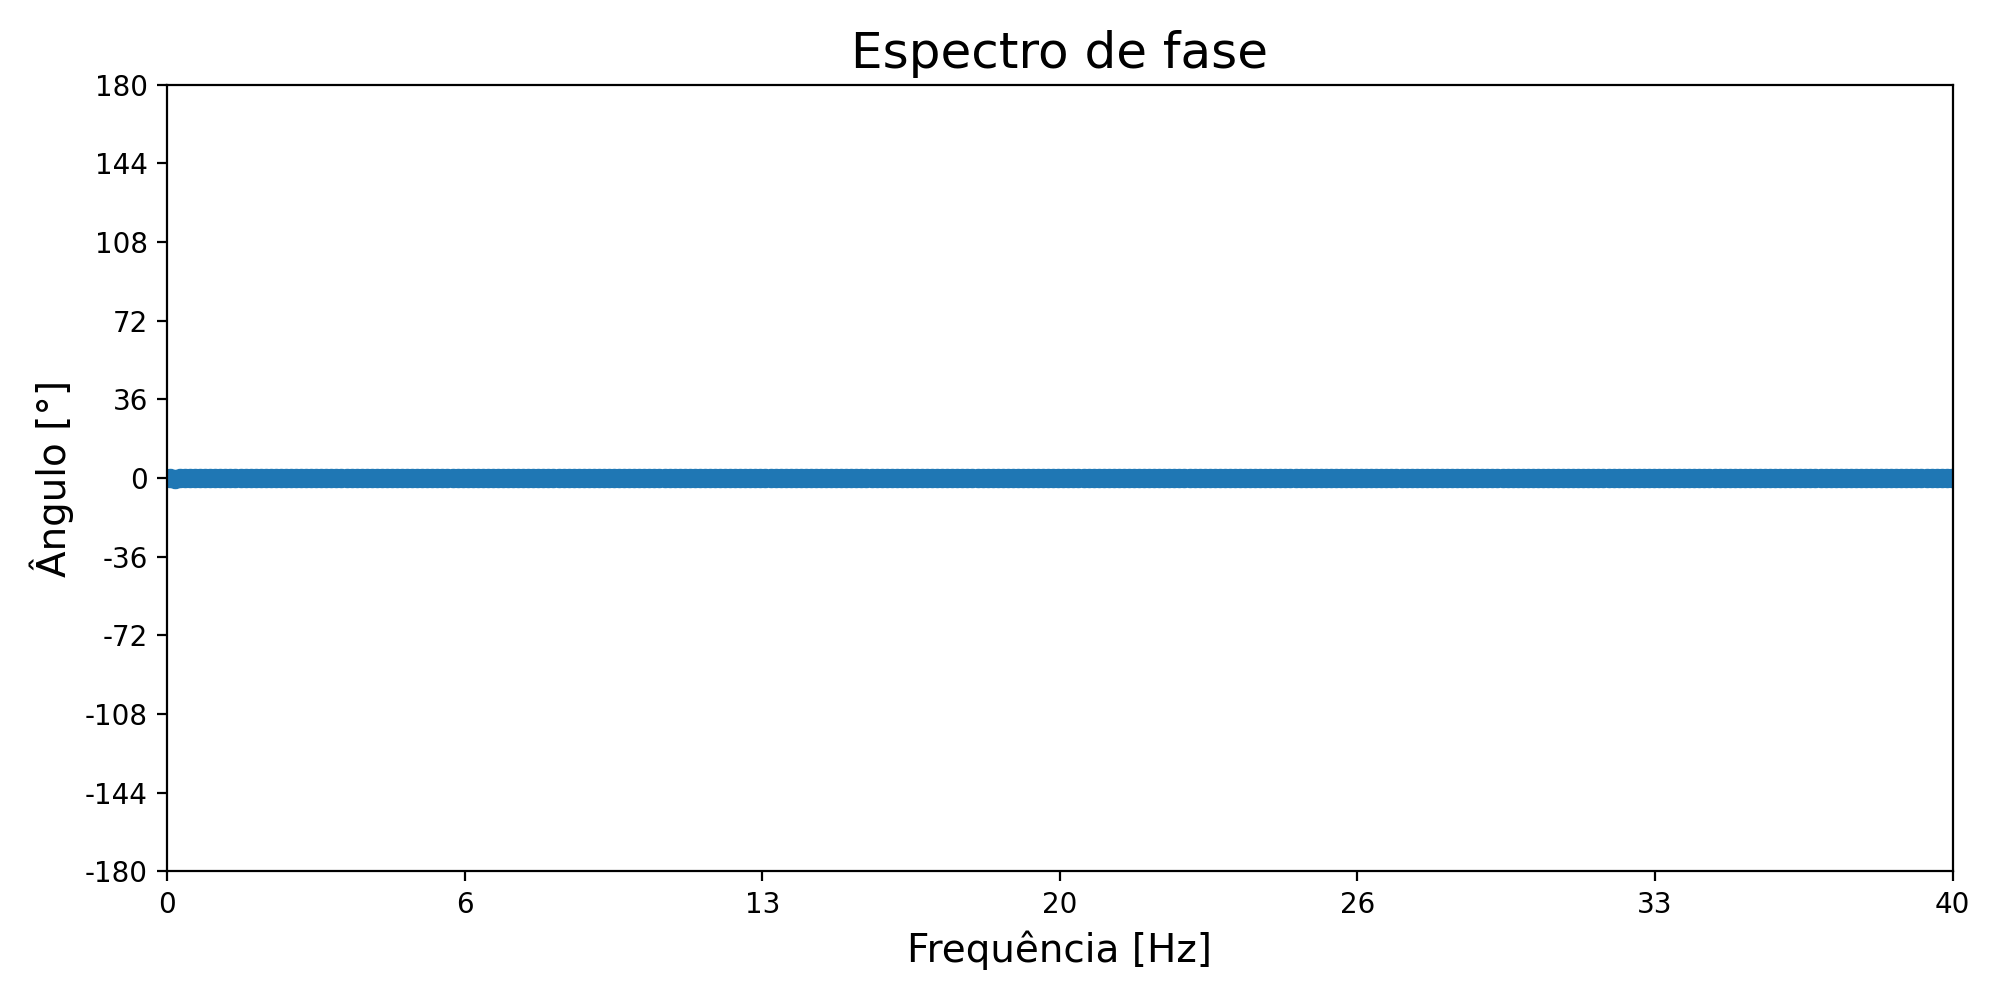
\includegraphics[width=8cm,height=4cm]{Imgs/Metodologia/ricker_zero_phase_d.png}}
		
	\caption{(a) Fonte Ricker centrada em zero. (b) Diagrama de polos e zeros. (c) Espectro de amplitudes e (d) espectro de fase.}
	\label{fig:ricker_zero_phase}
\end{figure}

\noindent Com a transformação da assinatura da fonte para fase mínima pode-se afirmar que a primeira reverberação que o receptor registrar será o tempo de trânsito alvo, pois utilizando a fonte de fase zero o tempo de trânsito alvo seria a metade do comprimento de onda registrado pelo sismograma. Comumente, em ensaios de tomografia, a equação eikonal é utilizada para gerar o dado observado, porém a abordagem de modelagem sísmica e seleção dos tempos de primeira chegada automatizados faz com que nenhum método de resolução eikonal seja privilegiado. Assim, os tempos de trânsito podem conter desvios causados pelo erro do algoritmo de seleção dos tempos de primeira chegada. 

Foi efetuada a modelagem sísmica para meios acústicos de densidade constante com a frequência máxima de 40 Hz. A discretização de 10 m do modelo de velocidade de referência foi considerada para todas as direções do espaço cartesiano. Para respeitar os limites de dispersão e estabilidade das diferenças finitas, a discretização temporal recebeu o parâmetro de 1 ms, totalizando 3 segundos completos de simulação. As bordas absortivas utilizando a equação \ref{cerjan} receberam o valor de 50 amostras com um fator atenuante de 0,0045. A figura \ref{fig:gather_example} mostra o dado típico gerado na simulação com a projeção dos tempos de trânsito calculados com a formulação de seleção automática. Os sismogramas são ordenados no domínio do receptor, então a Figura \ref{fig:gather_example} ilustra o sismograma da estação 176, a última efetuada na simulação.     

\begin{figure}[H]
	\centering
	\subfloat[]{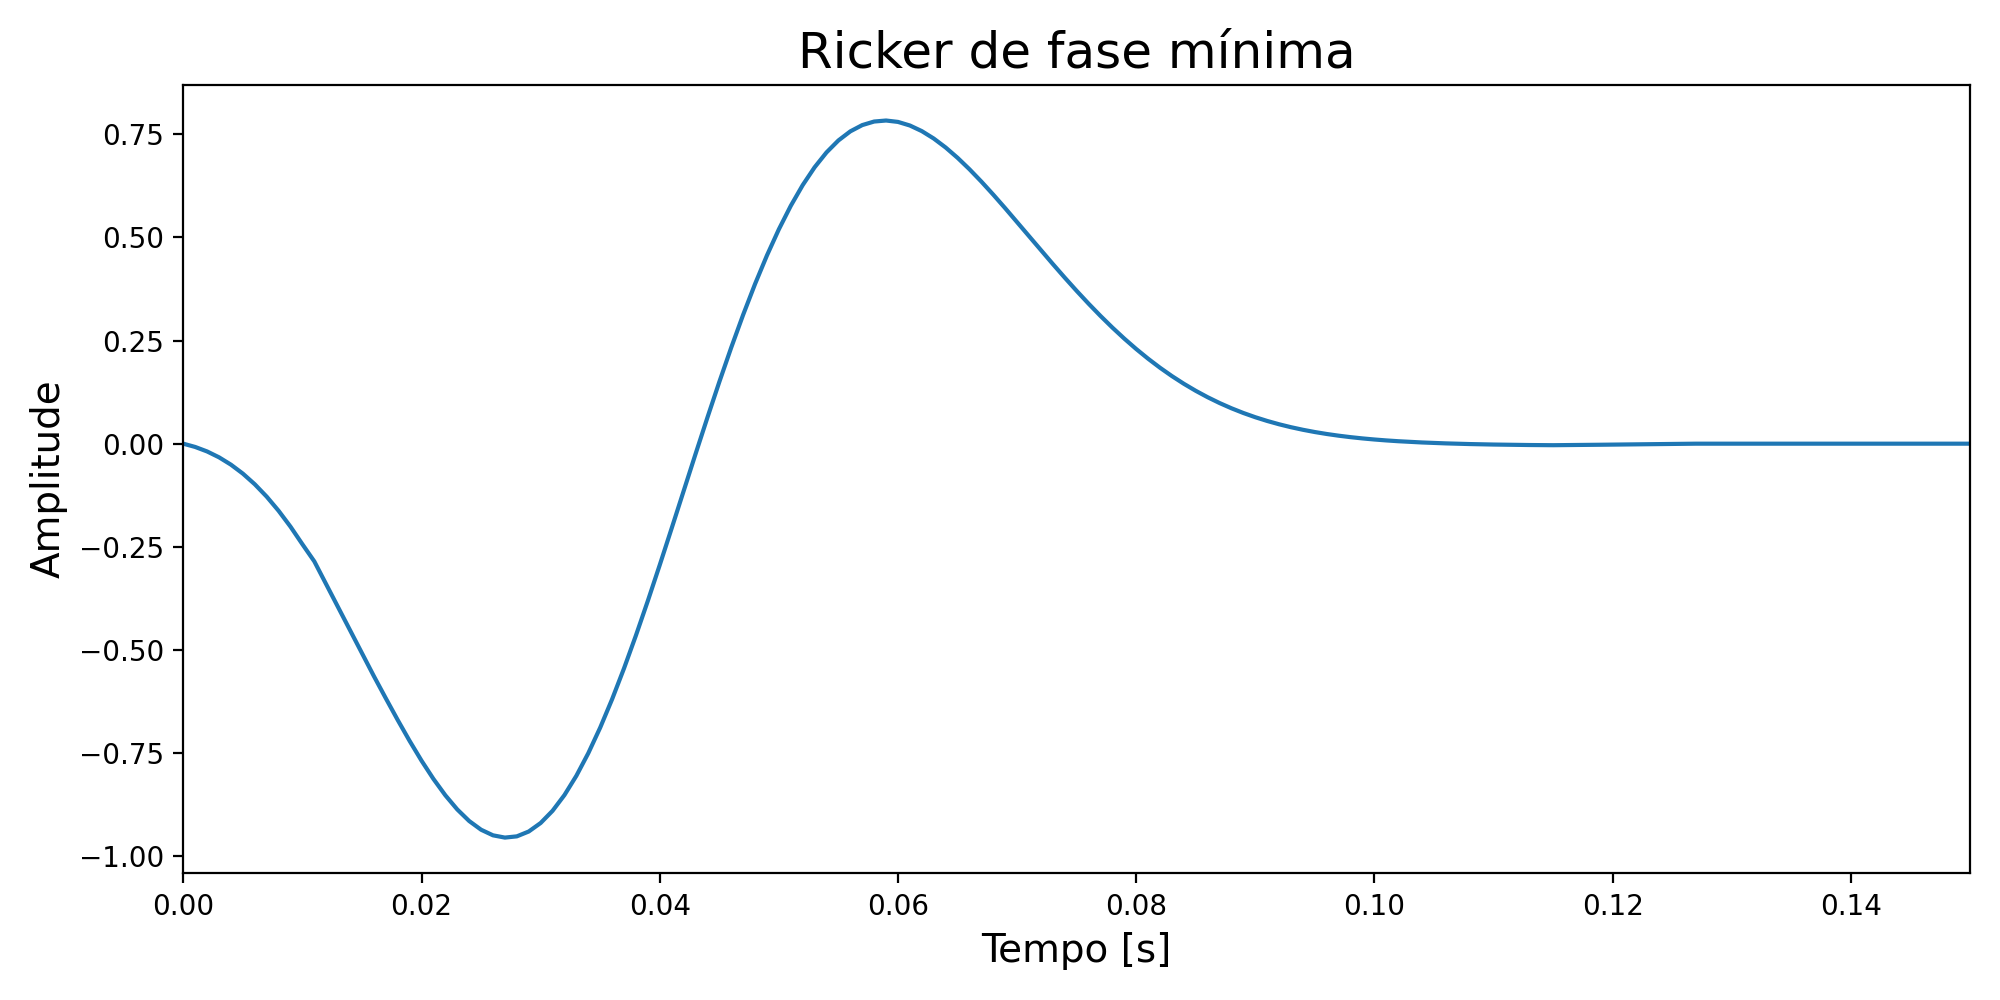
\includegraphics[width=8cm,height=4cm]{Imgs/Metodologia/ricker_min_phase_a.png}}
	\subfloat[]{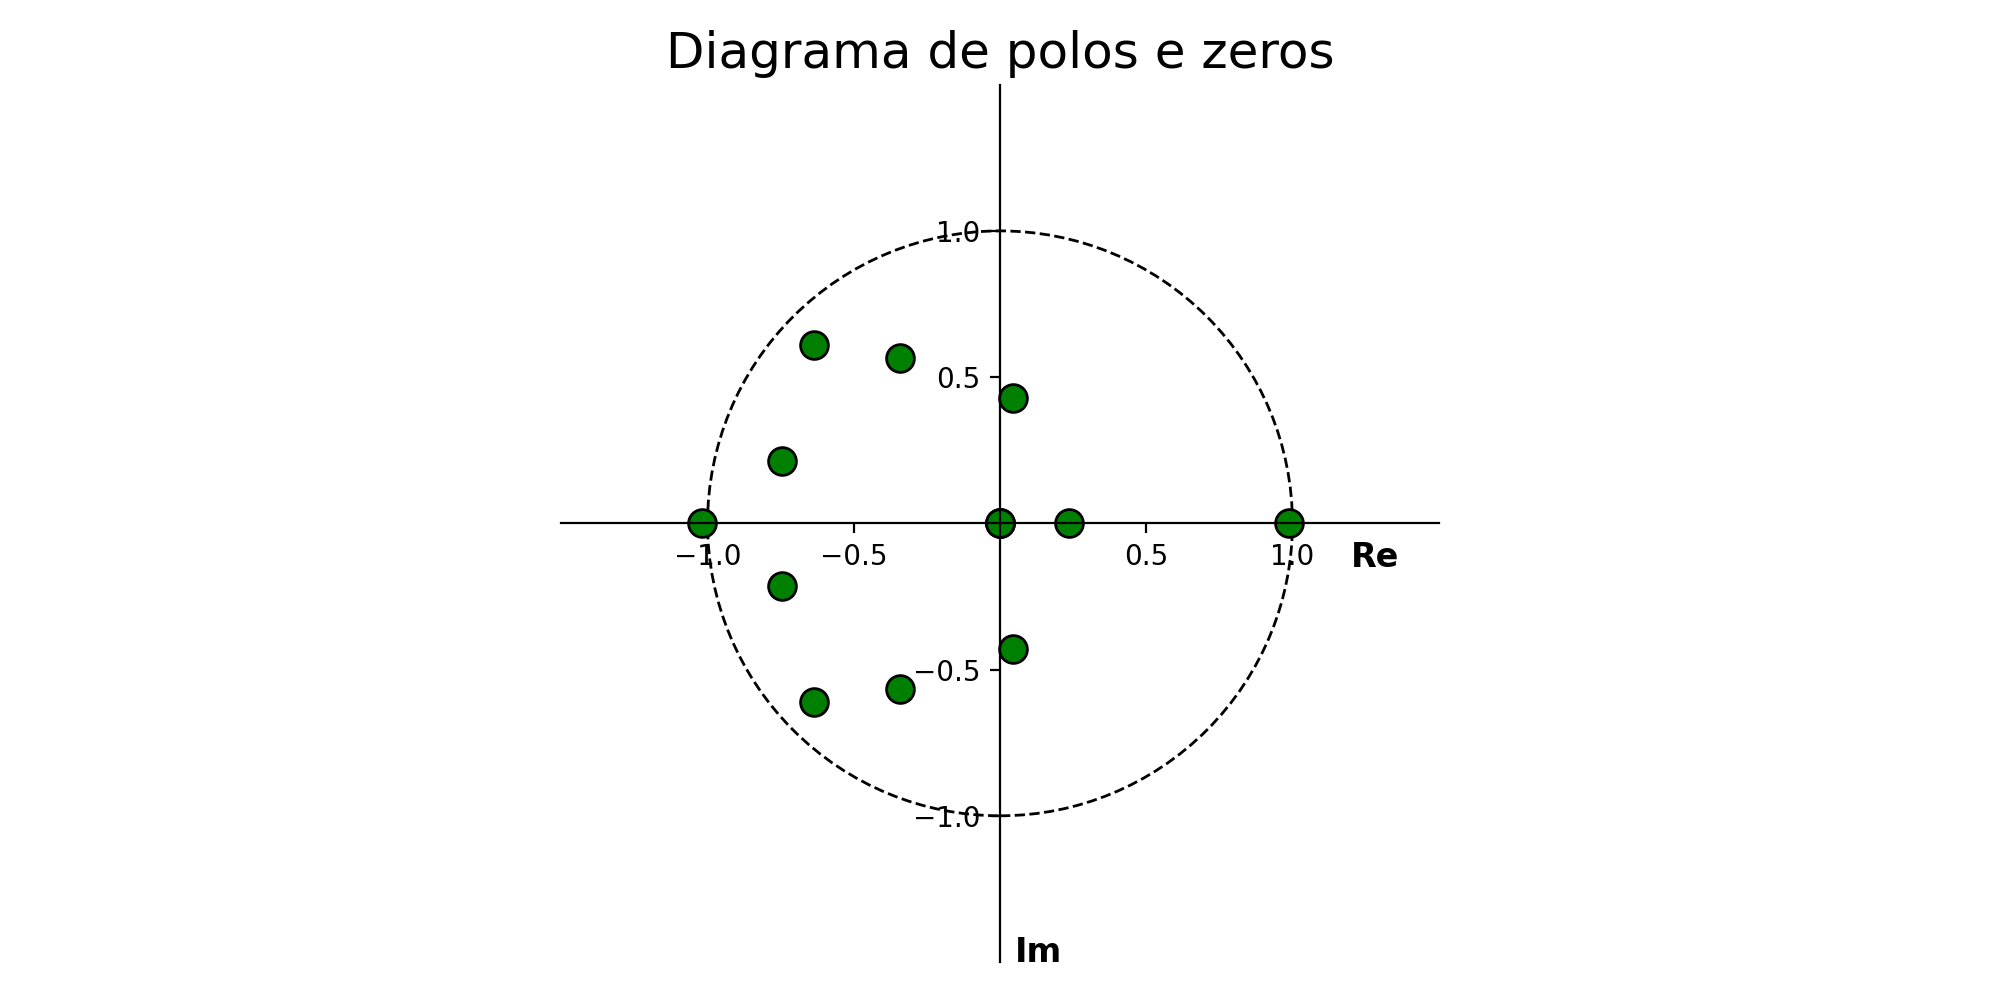
\includegraphics[width=8cm,height=4cm]{Imgs/Metodologia/ricker_min_phase_b.png}}
	
	\subfloat[]{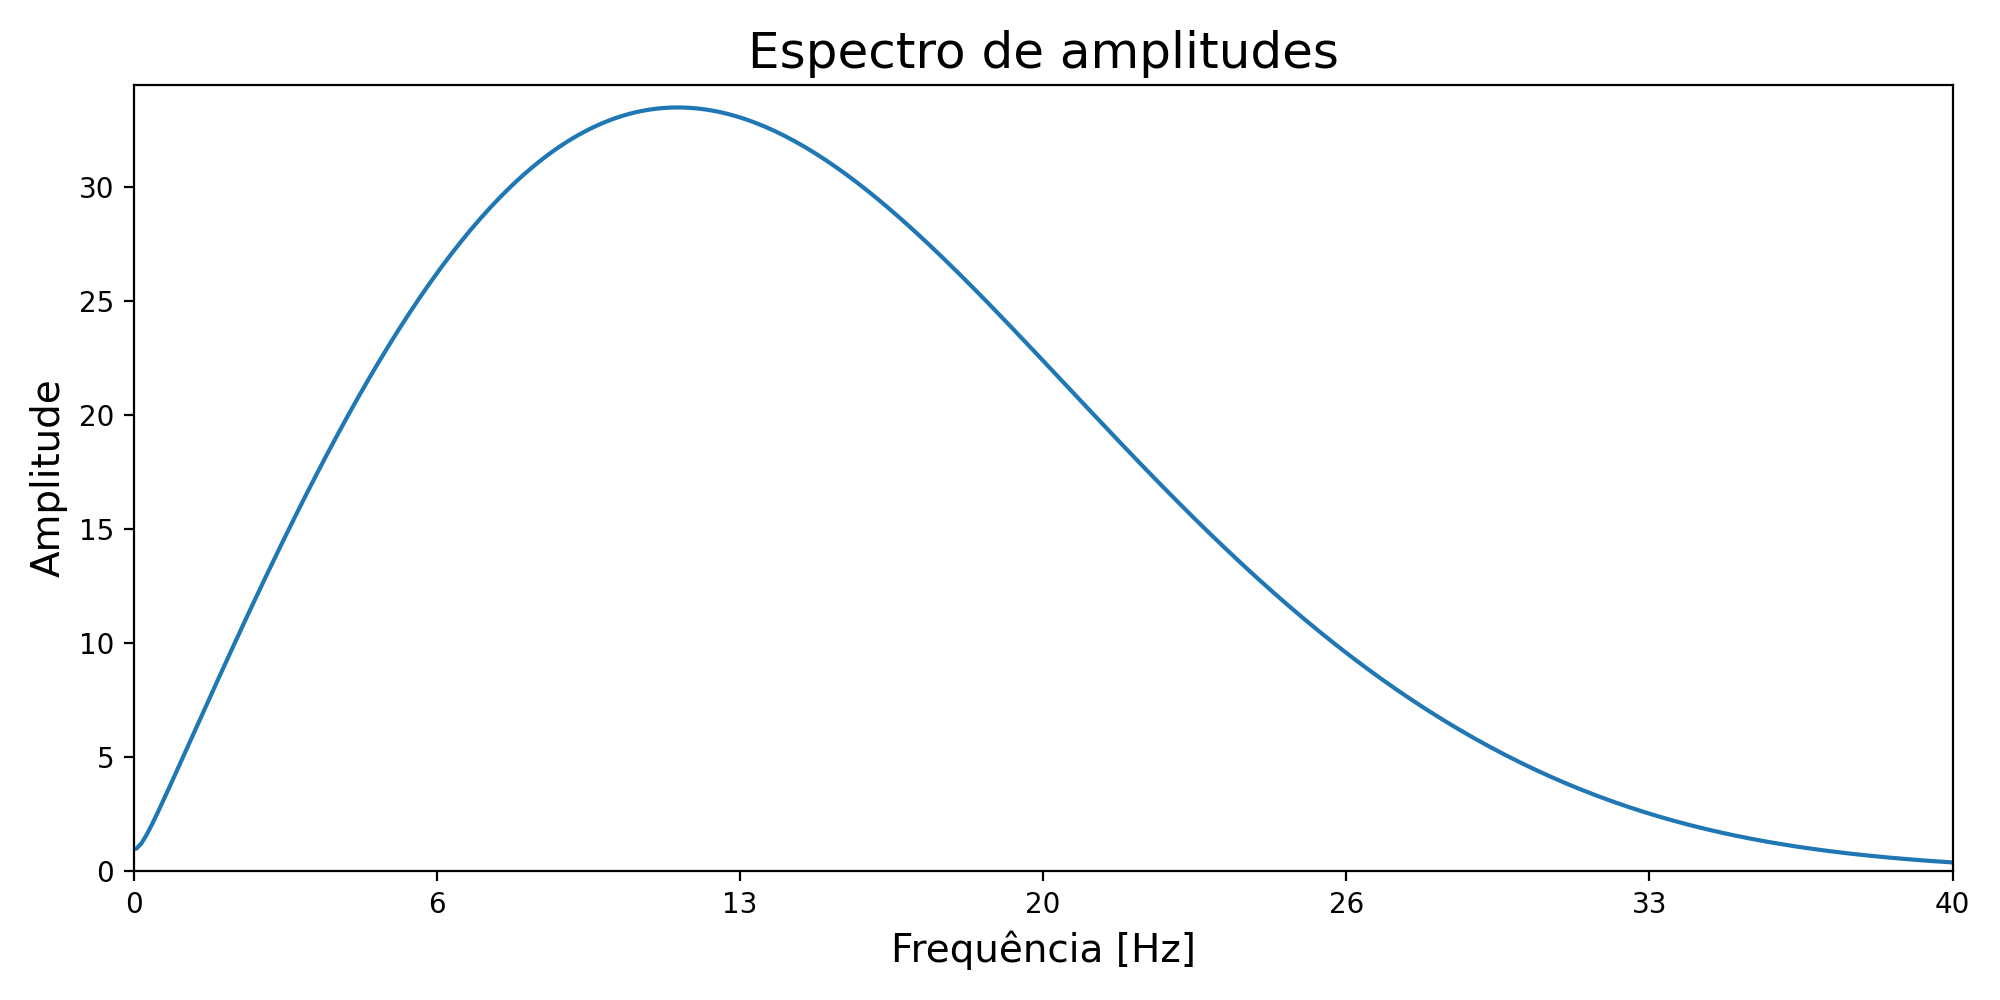
\includegraphics[width=8cm,height=4cm]{Imgs/Metodologia/ricker_min_phase_c.png}}
	\subfloat[]{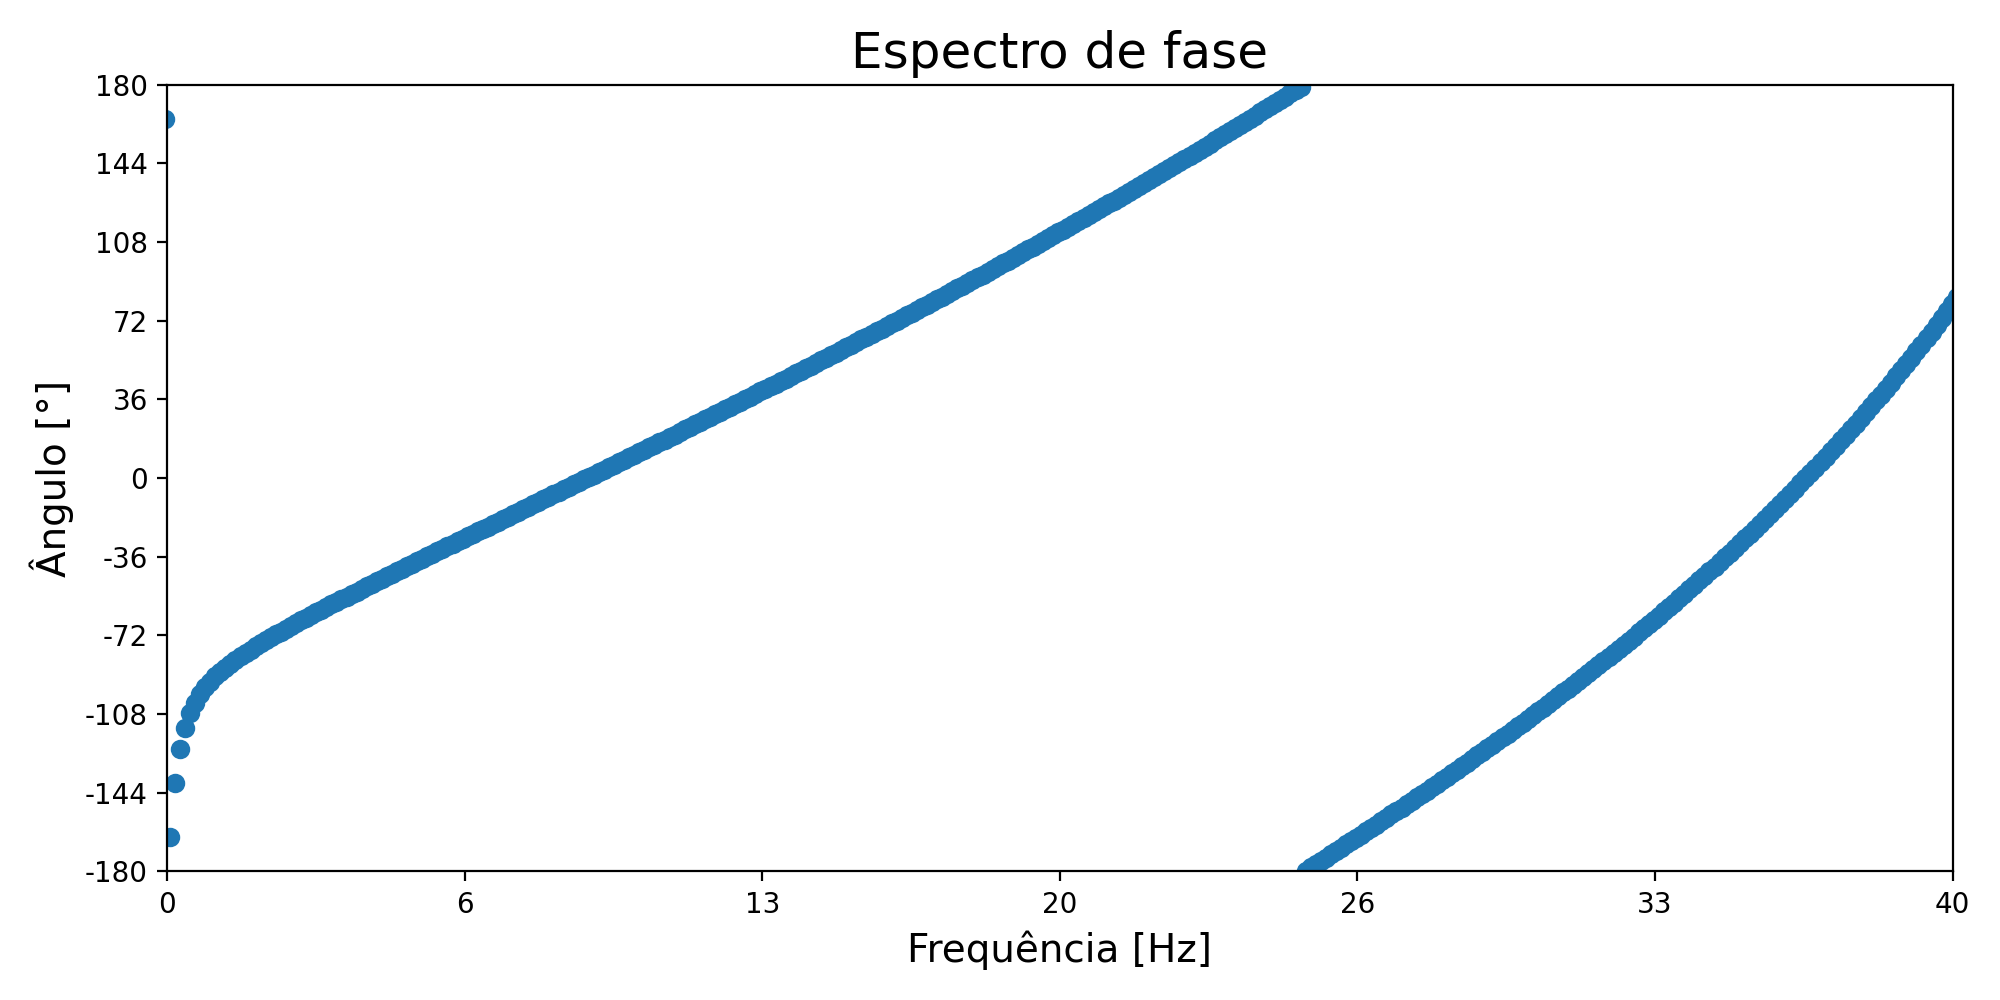
\includegraphics[width=8cm,height=4cm]{Imgs/Metodologia/ricker_min_phase_d.png}}
	
	\caption{Fonte Ricker inicializando de zero. (b) Diagrama de polos e zeros. (c) Espectro de amplitudes e (d) espectro de fase.}
	\label{fig:ricker_min_phase}
\end{figure}

\begin{figure}[H]
	\centering
	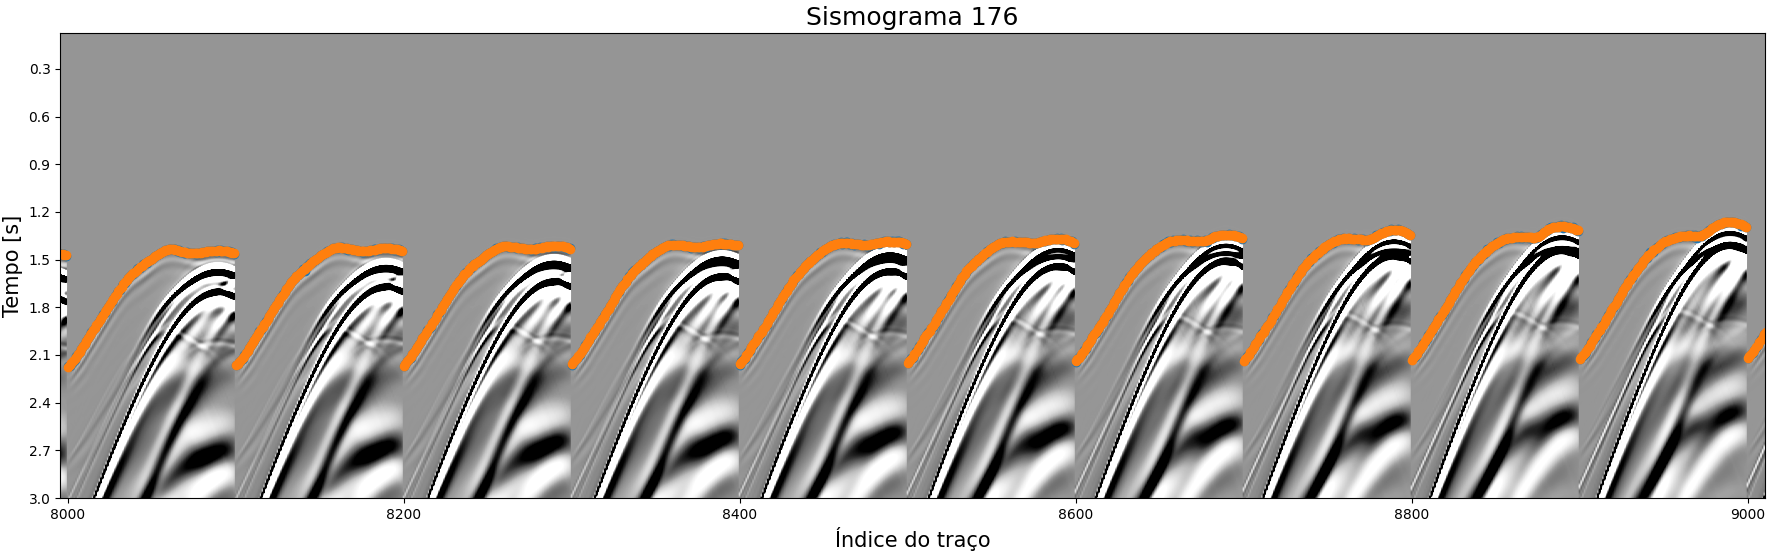
\includegraphics[width=16cm,height=5cm]{Imgs/Metodologia/gather_example.png}
	\caption{Seleção da primeira chegada ilustrada em alguns sismogramas da estação 176.}
	\label{fig:gather_example}	
\end{figure}

As Figuras \ref{fig:gather_picking_near}, \ref{fig:gather_picking_mid} e \ref{fig:gather_picking_far} ilustram 100 traços do sismograma no domínio do receptor para a primeira estação, representando as distâncias próximas, médias e longas entre fonte e receptores. Para essas visualizações, uma linha de tiros na direção $y$ foi retirada nas posições 10, 80 e 135. Observando o mapa da geometria mostrado na Figura \ref{fig:complete_geometry}, o primeiro sismograma se localiza na posição mais próxima da origem do mapa, então, a linha 10 se posiciona com a direção $x$ fixa em 500 m, a linha 80 na posição 4 km e a linha 135 na posição 6,8 km, incluindo todas as fontes na direção $y$. 

\begin{figure}[H]
	\centering
	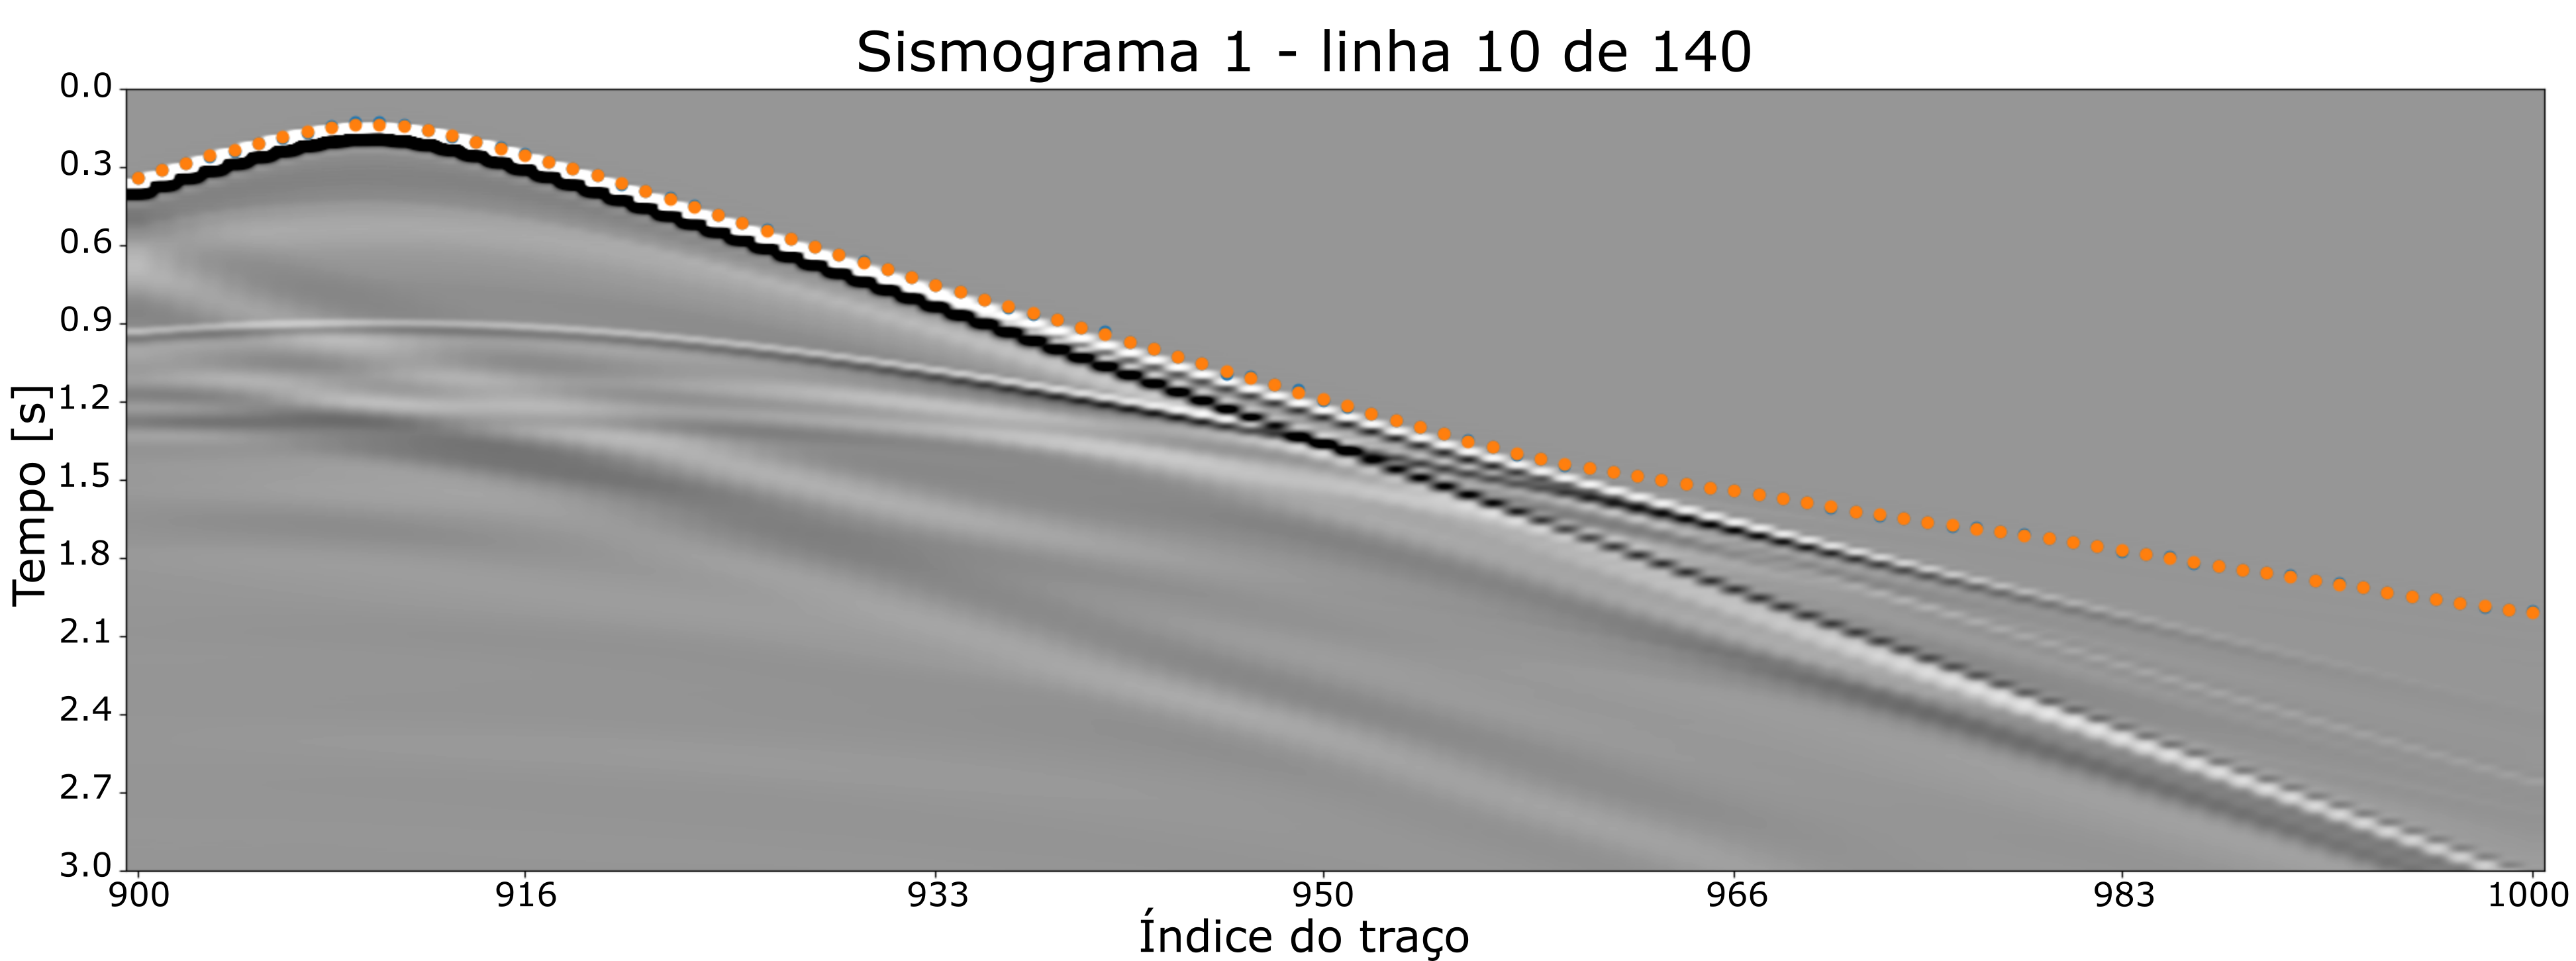
\includegraphics[width=16cm,height=6cm]{Imgs/Metodologia/linha10_sismo1.png}
	\caption{Seleção da primeira chegada em um sismograma de curto afastamento entre fonte e receptor. Presença predominante da onda direta. Primeira chegada denotada como pontos laranjas, recuperadas por seleção automática.}
	\label{fig:gather_picking_near}	
\end{figure}

\begin{figure}[H]
	\centering
	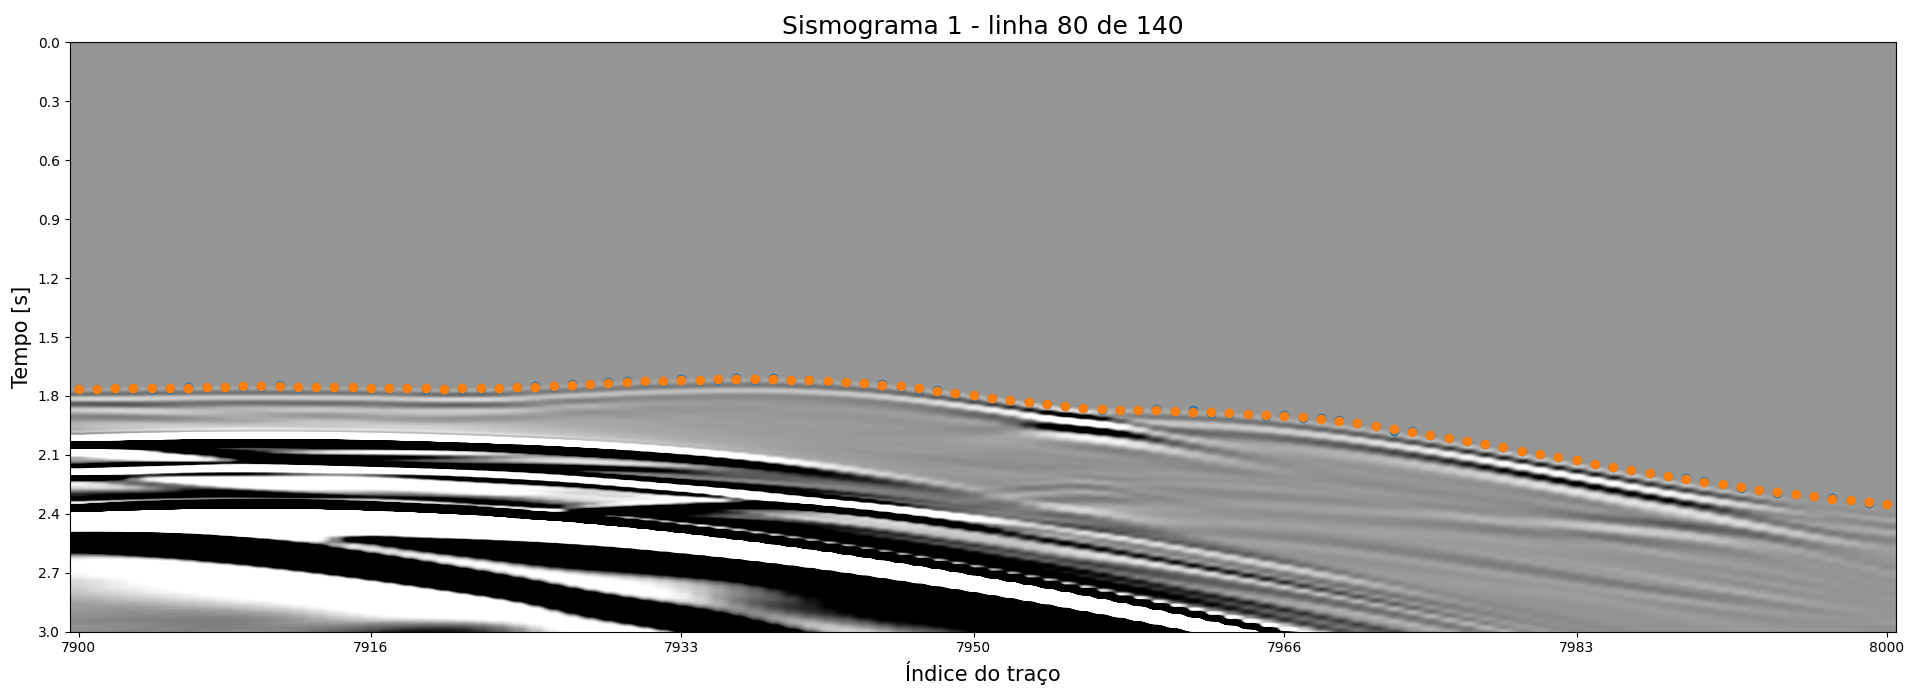
\includegraphics[width=16cm,height=6cm]{Imgs/Metodologia/linha80_sismo1.png}
	\caption{Seleção da primeira chegada em um sismograma de médio afastamento entre fonte e receptor. Presença predominante de refrações.}
	\label{fig:gather_picking_mid}	
\end{figure}

O método de seleção automática das primeiras chegadas depende de certos parâmetros para seu funcionamento, como mostrado na equação \ref{automatic_picking}. A janela escolhida para a seleção automática foi de 10 ms, baseado no trabalho de \citeonline{qin2021first} onde se utilizou janelas entre 30 a 10 ms nos exemplos mostrados. Por consequência do dado observado ser completamente sintético, não contendo ruído instrumental ou ambiental, o algoritmo analítico se mostrou eficiente. Contudo algumas instabilidades imperceptíveis nos resultados foram encontradas e removidas com a filtragem de \citeonline{savitzky1964smoothing} de segunda ordem com janela de 11 amostras.   

\begin{figure}[H]
	\centering
	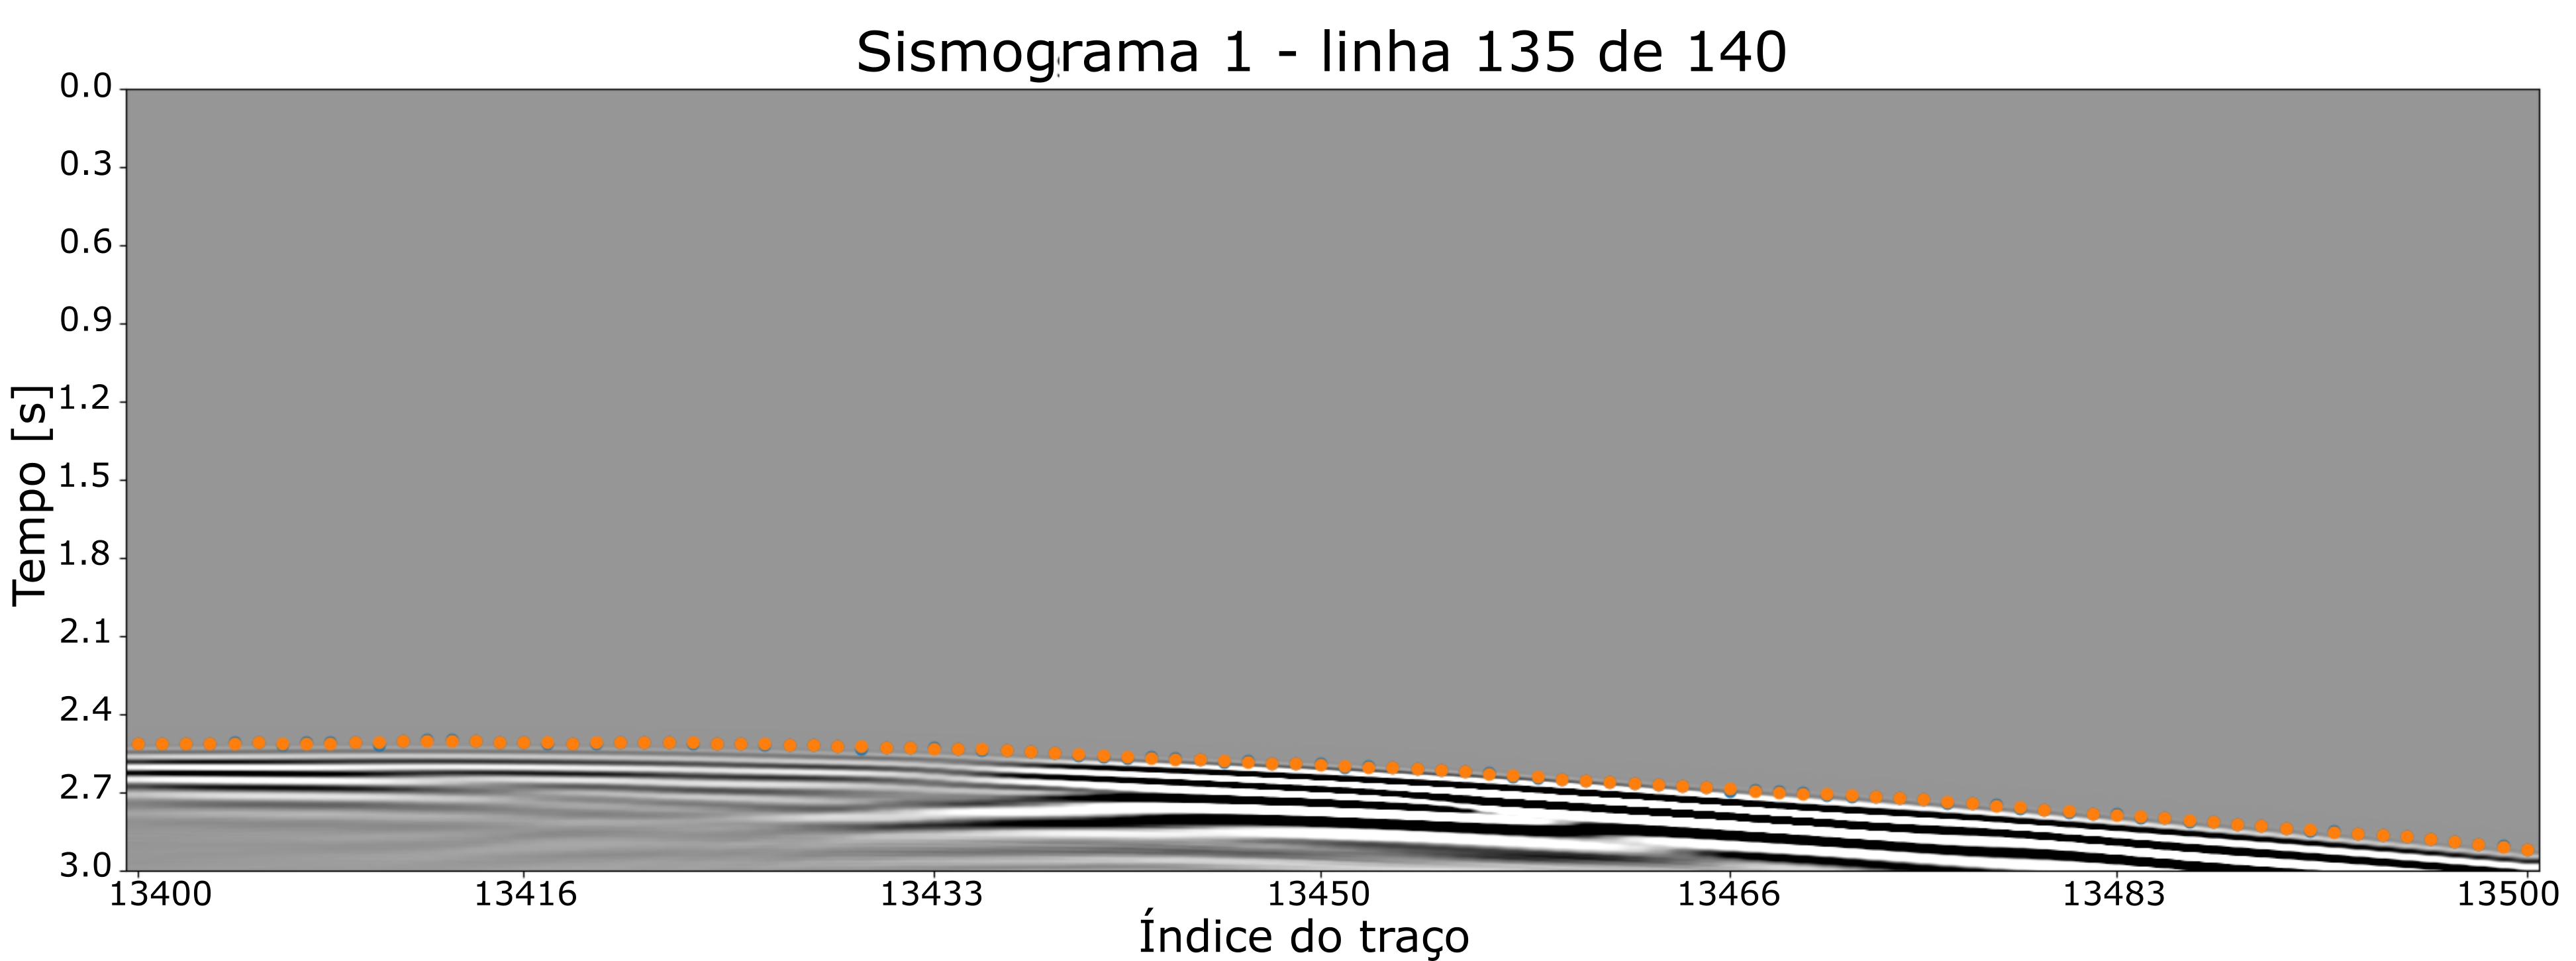
\includegraphics[width=16cm,height=6cm]{Imgs/Metodologia/linha135_sismo1.png}
	\caption{Seleção da primeira chegada em um sismograma de longo afastamento entre fonte e receptor. Somente refrações selecionadas.}
	\label{fig:gather_picking_far}	
\end{figure}

\subsection{Configurações do esquema de inversão}

O modelo de velocidade no processo tomográfico foi discretizado por blocos. A discretização do modelo na modelagem, ou seja, na propagação da equação eikonal, pode ser diferente da discretização no processo de inversão. Então, o experimento foi dividido em duas etapas: uma inversão com malha esparsa e uma com malha refinada. Para ambos esquemas o modelo de velocidade se manteve com o mesmo espaçamento regular de 20 metros. A malha de inversão esparsa possui parâmetros de discretização 100, 300 e 300 metros para as direções $z$, $x$ e $y$, respectivamente. A malha de inversão refinada possui espaçamentos de 20, 100 e 100 metros para as direções $z$, $x$ e $y$, respectivamente. Para reconhecimento regional do modelo, 5 iterações foram alocadas para o processo tomográfico de malha esparsa. Na tentativa de realçar os detalhes no modelo, 10 iterações foram alocadas para o processo tomográfico de malha refinada. A regularização alocada foi a Tikhonov de segunda ordem utilizando os parâmetros escalares de $10^5$ e $10^4$ para as inversões de malha esparsa e refinada, respectivamente. A modificação da ordem do parâmetro de regularização possui influência com a magnitude da matriz de modelagem direta $G_{N\times M}$, definindo a distância percorrida por raios de cada célula do modelo para cada raio. A grandeza da matriz $G_{N\times M}$ atinge um valor constante para a quantidade de dados $N = 2464000$, sendo as equações do sistema linear. Em relação aos parâmetros do modelo $M$, foi utilizado $M = 4488$ e $M = 184671$ para a malha esparsa e refinada, respectivamente.   







